\section{Függelék}
\label{sec:fuggelek}

\begin{thebibliography}{1}
	
	\bibitem{SAW} \textbf{SF2446E} \url{https://www.rfmi.co/pdf/Datasheet/sf2446e.pdf}
	
	\bibitem{ADL} \textbf{ADL5523}
	\url{https://www.analog.com/media/en/technical-documentation/data-sheets/ADL5523.pdf}
	
	\bibitem{PGA} \textbf{PGA-103+} \url{https://www.minicircuits.com/pdfs/PGA-103+.pdf}
	
	\bibitem{PGA_comp} \textbf{PGA-103+ kompenzáló hálózat} \url{https://www.minicircuits.com/app/AN60-064.pdf}
	
	\bibitem{90es_SMA} \textbf{$90^{\circ}$-os SMA csatlakozó}
	\url{https://lomex.hu/hu/webshop/#page,0/search,43-28-29/stype,1}
	
	\bibitem{L1} \textbf{330\,nH tekercs}
	\url{https://lomex.hu/hu/webshop/#page,0/search,93-00-72/stype,1}
	
	\bibitem{R1} \textbf{150\,$\Omega$ ellenállás}
	\url{https://lomex.hu/hu/webshop/#page,0/search,80-10-76/stype,1}
	
	\bibitem{C1} \textbf{330\,pF kondenzátor}
	\url{https://lomex.hu/hu/webshop/#page,0/search,82-07-43/stype,1}
	
	\bibitem{doboz} \textbf{Árnyékolódoboz}
	\url{https://hu.mouser.com/ProductDetail/Bud-Industries/CU-5470/?qs=J02F3jFhwzOGRdkfRTc5YA%3D%3D}
	
	\bibitem{egyenes_SMA} \textbf{Egyenes SMA csatlakozó}
	\url{https://hu.mouser.com/ProductDetail/Linx-Technologies/CONSMA008-G/?qs=vLWxofP3U2zf85vM2YDg9g%3D%3D}
	
	\bibitem{dioda} \textbf{Dióda}
	\url{https://lomex.hu/hu/webshop/#page,0/search,83-01-43/stype,1}


\end{thebibliography}

\newpage

\subsection{Mérési eredmények grafikusan}

\begin{figure}[!ht]
	\centering
	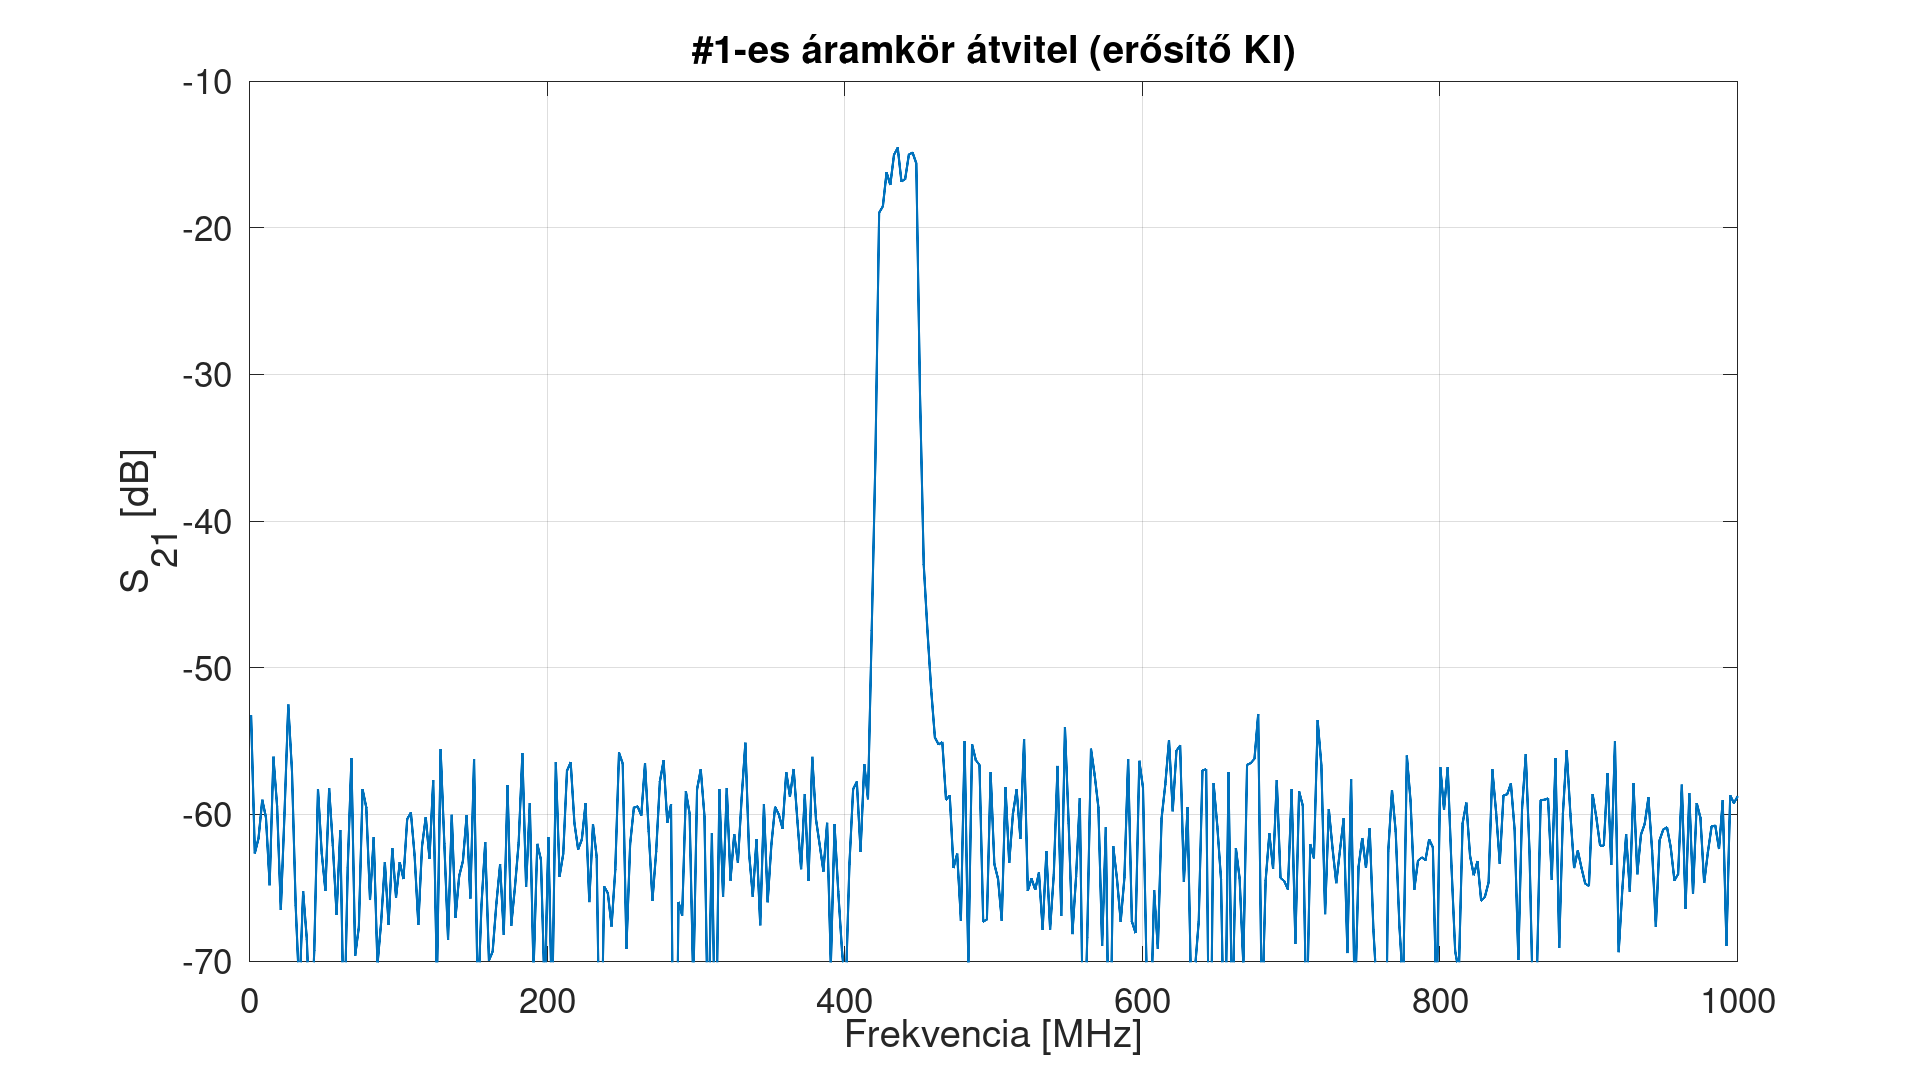
\includegraphics[keepaspectratio, width=\textwidth]{aramkor1_1.png}
	\caption{\#1-es erősítő 1\,MHz - 1\,GHz, erősítő KI}
	\label{fig:meres1}
\end{figure}

\begin{figure}[!ht]
	\centering
	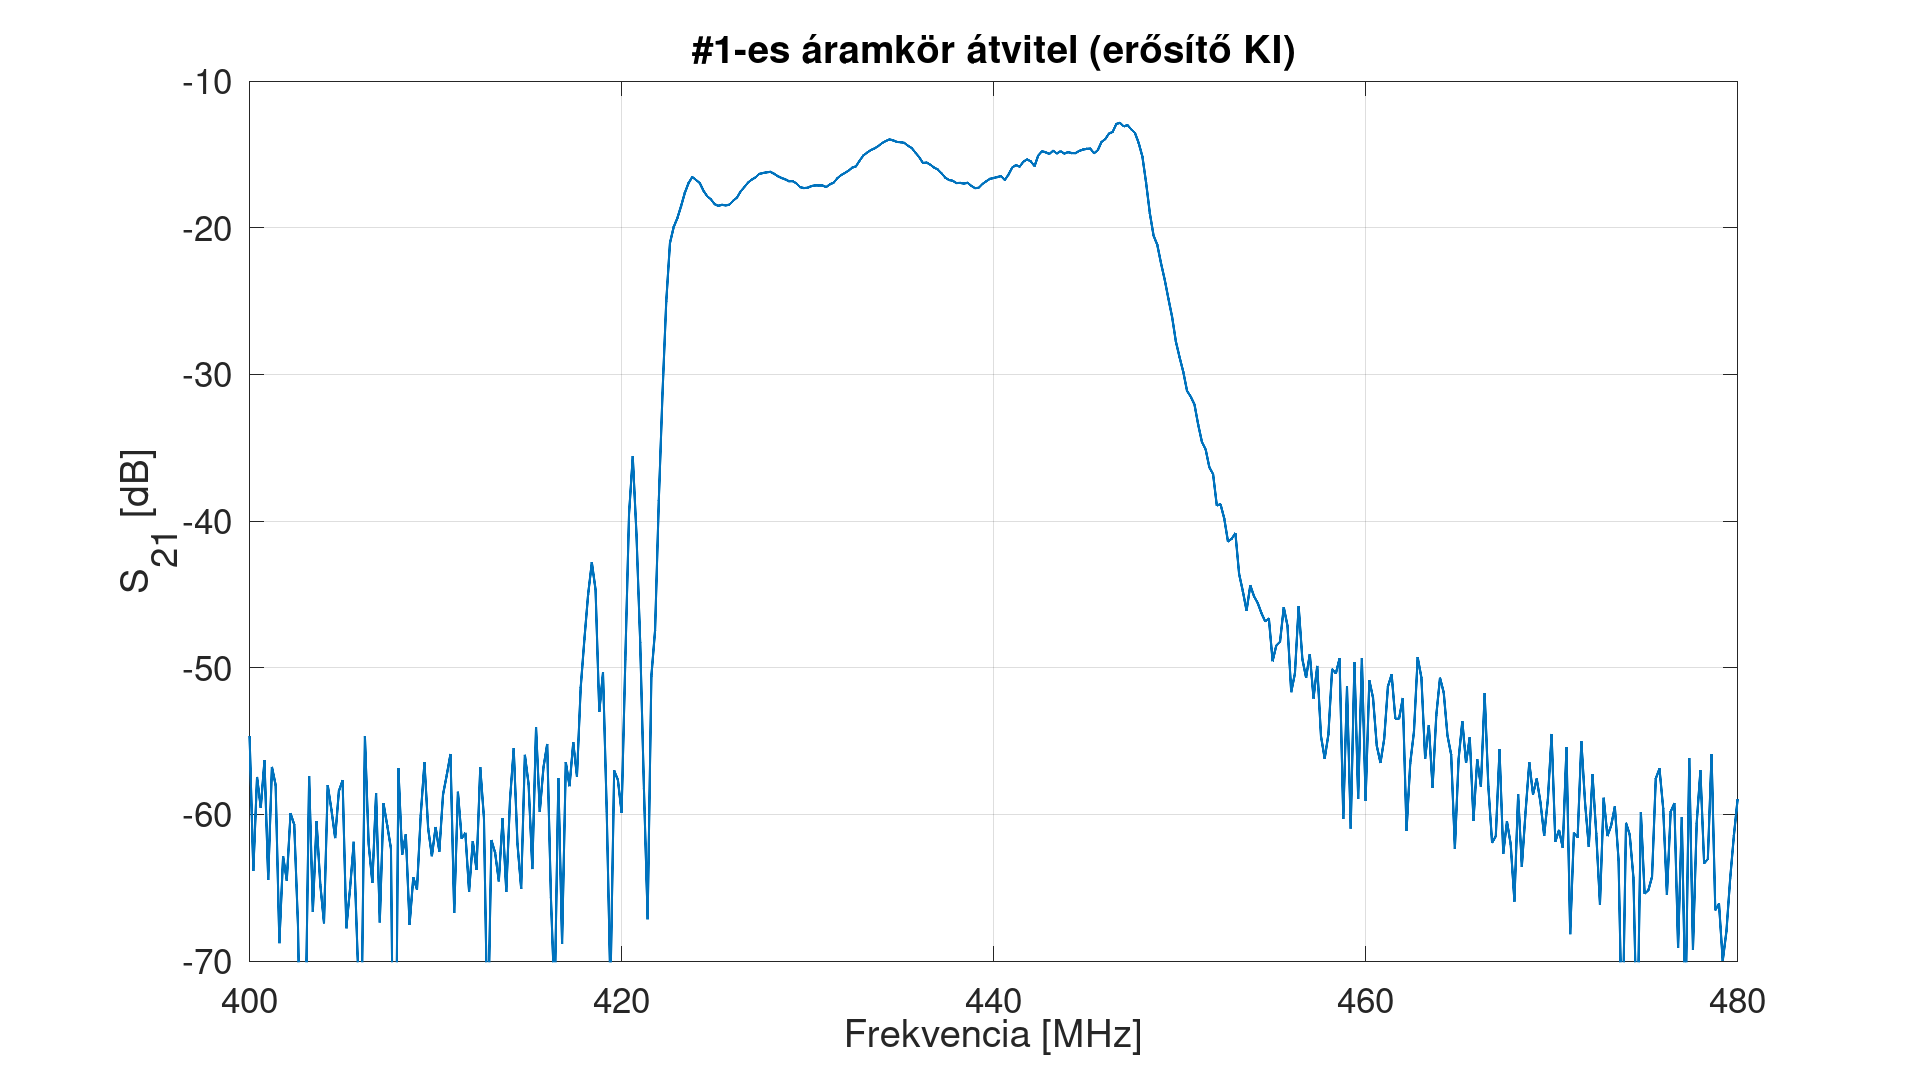
\includegraphics[keepaspectratio, width=\textwidth]{aramkor1_2.png}
	\caption{\#1-es erősítő 400\,MHz - 480\,MHz, erősítő KI}
	\label{fig:meres2}
\end{figure}

\begin{figure}[!ht]
	\centering
	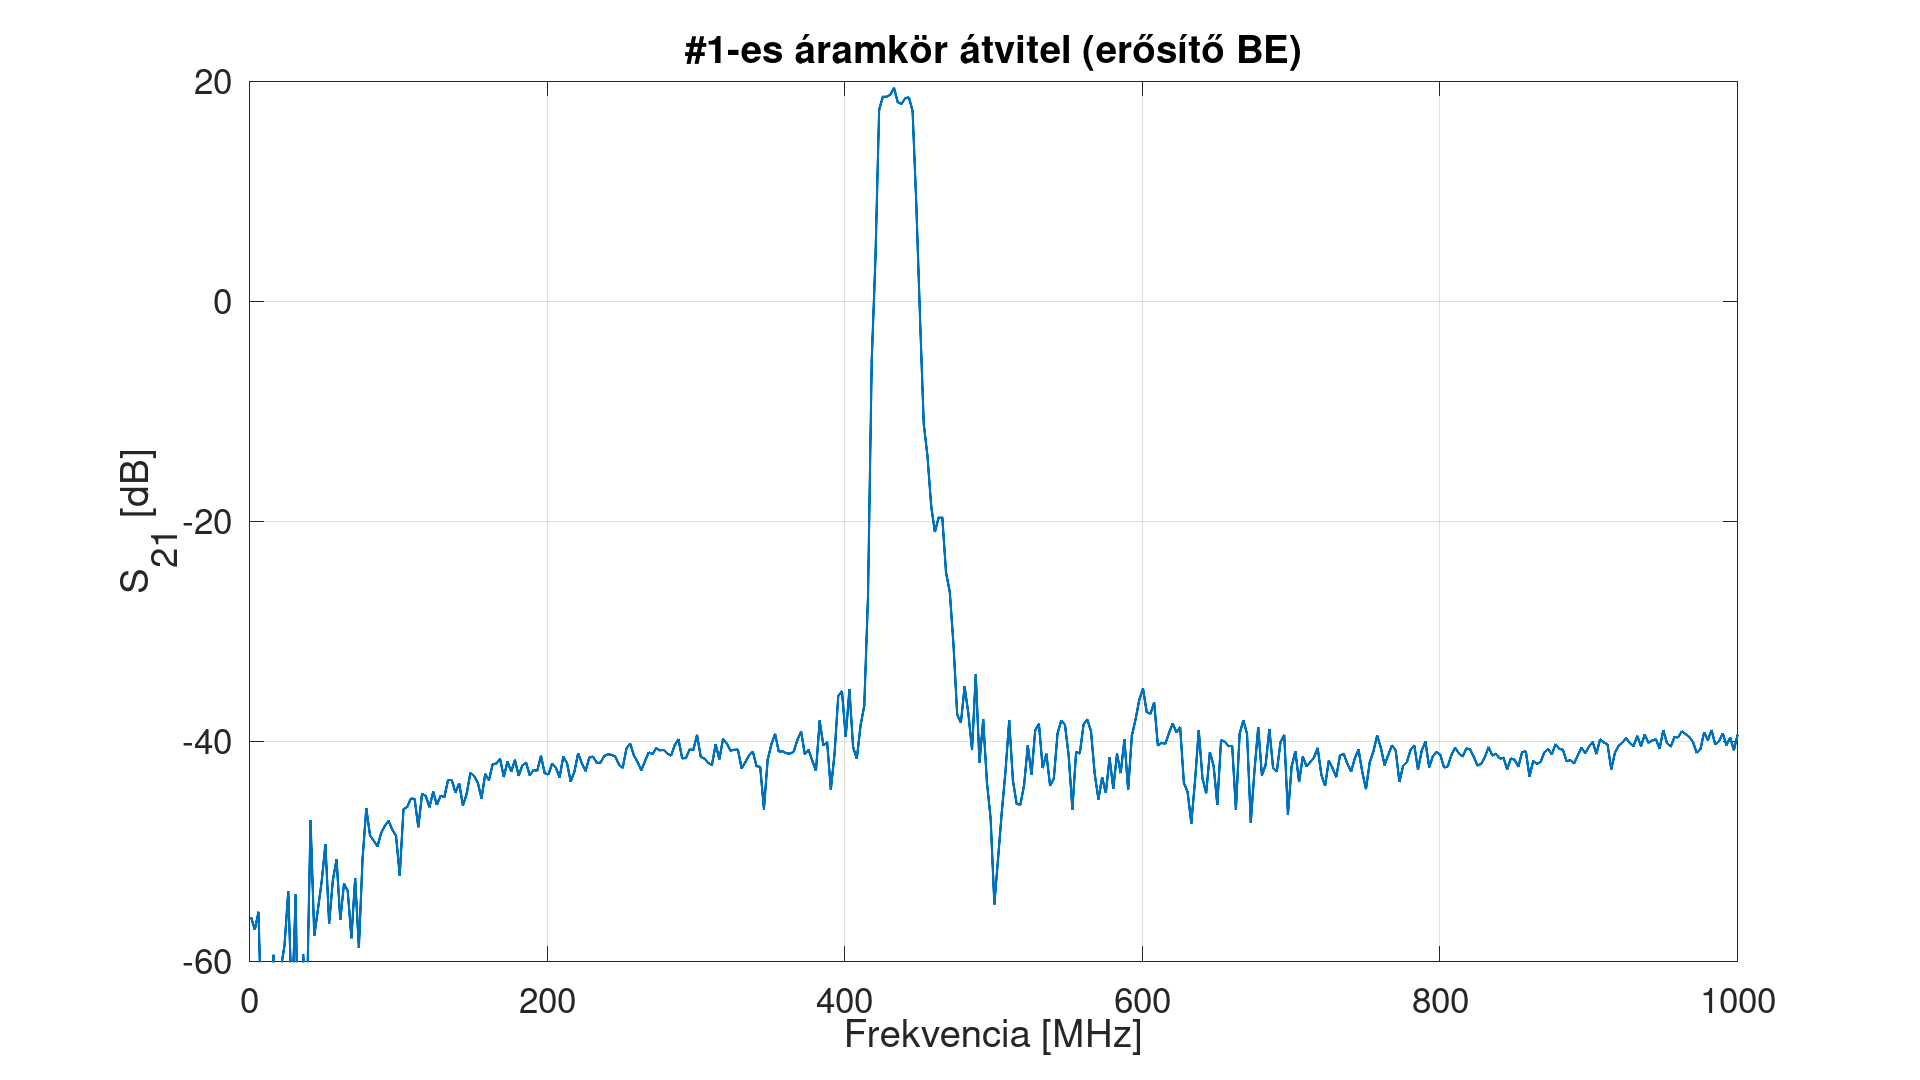
\includegraphics[keepaspectratio, width=\textwidth]{aramkor1_3.png}
	\caption{\#1-es erősítő 1\,MHz - 1\,GHz, erősítő BE}
	\label{fig:meres3}
\end{figure}

\begin{figure}[!ht]
	\centering
	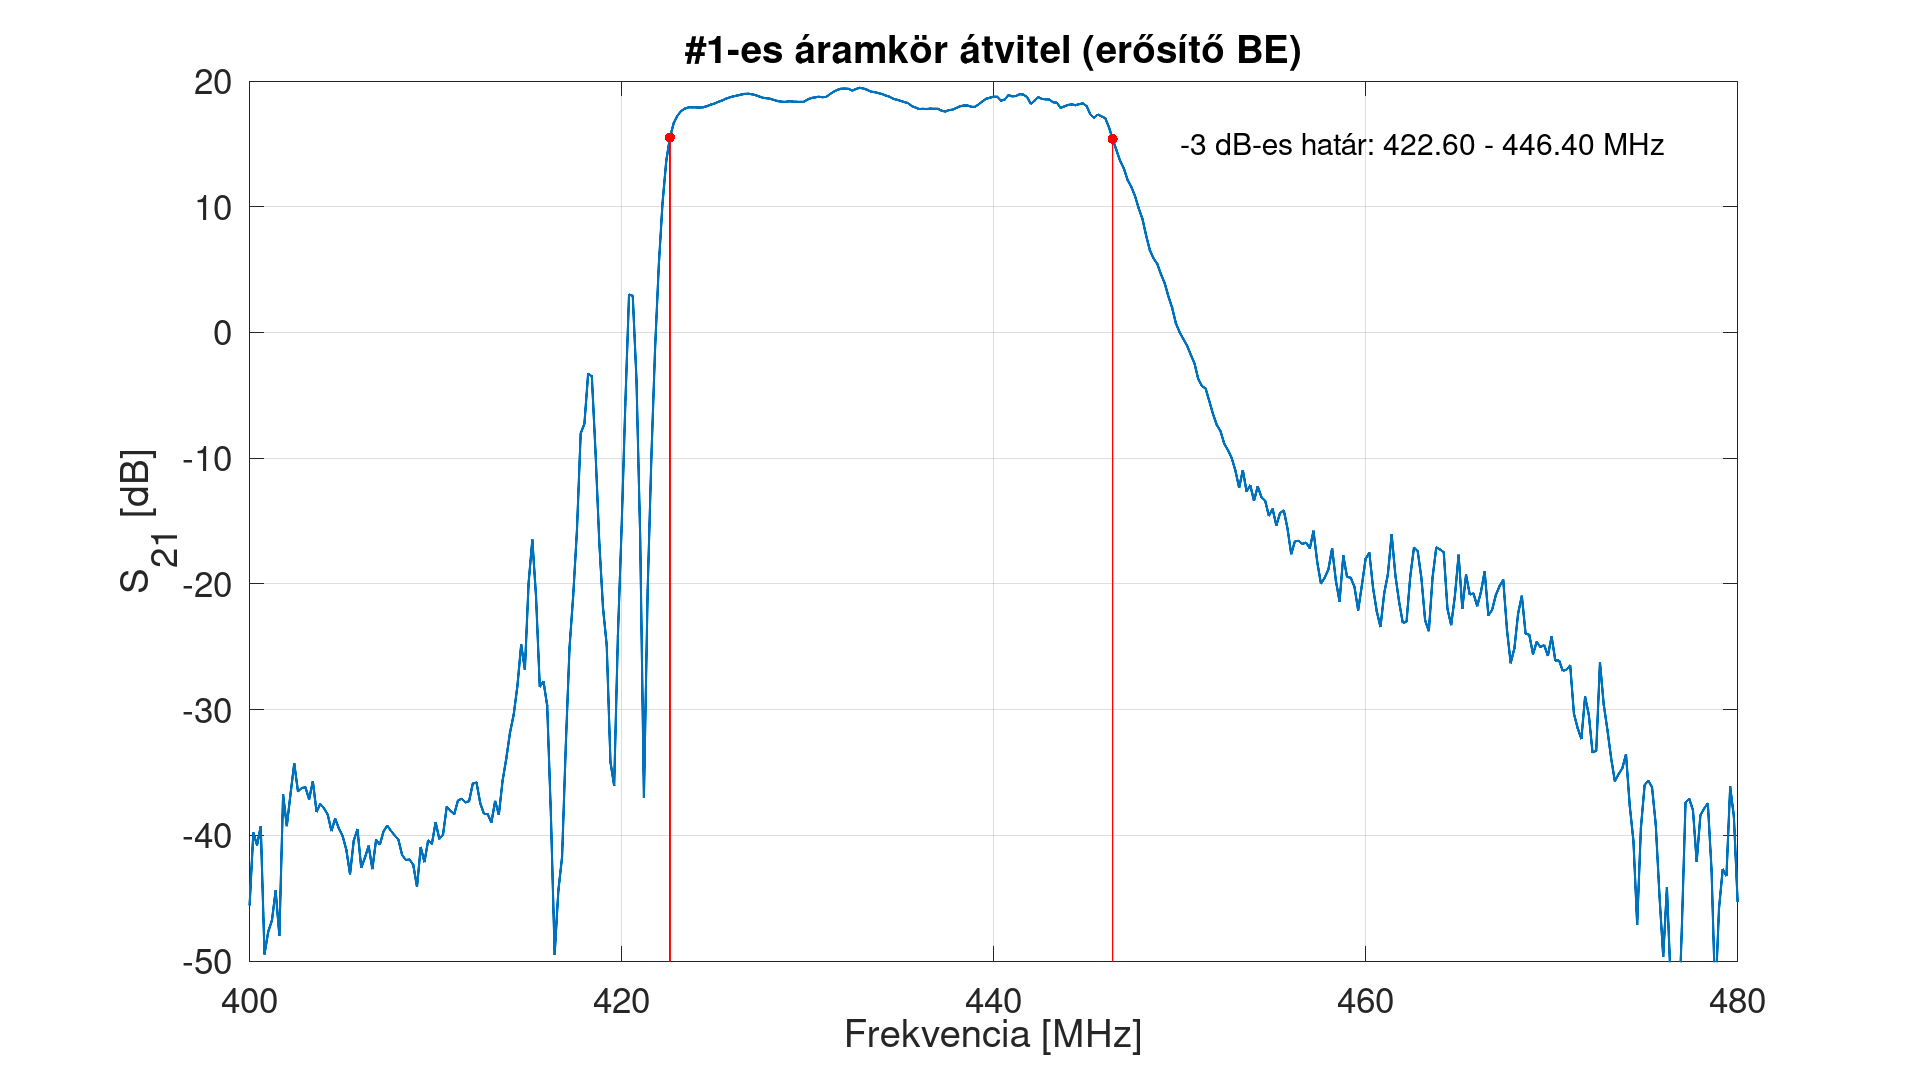
\includegraphics[keepaspectratio, width=\textwidth]{aramkor1_4.png}
	\caption{\#1-es erősítő 400\,MHz - 480\,MHz, erősítő BE}
	\label{fig:meres4}
\end{figure}



\begin{figure}[!ht]
	\centering
	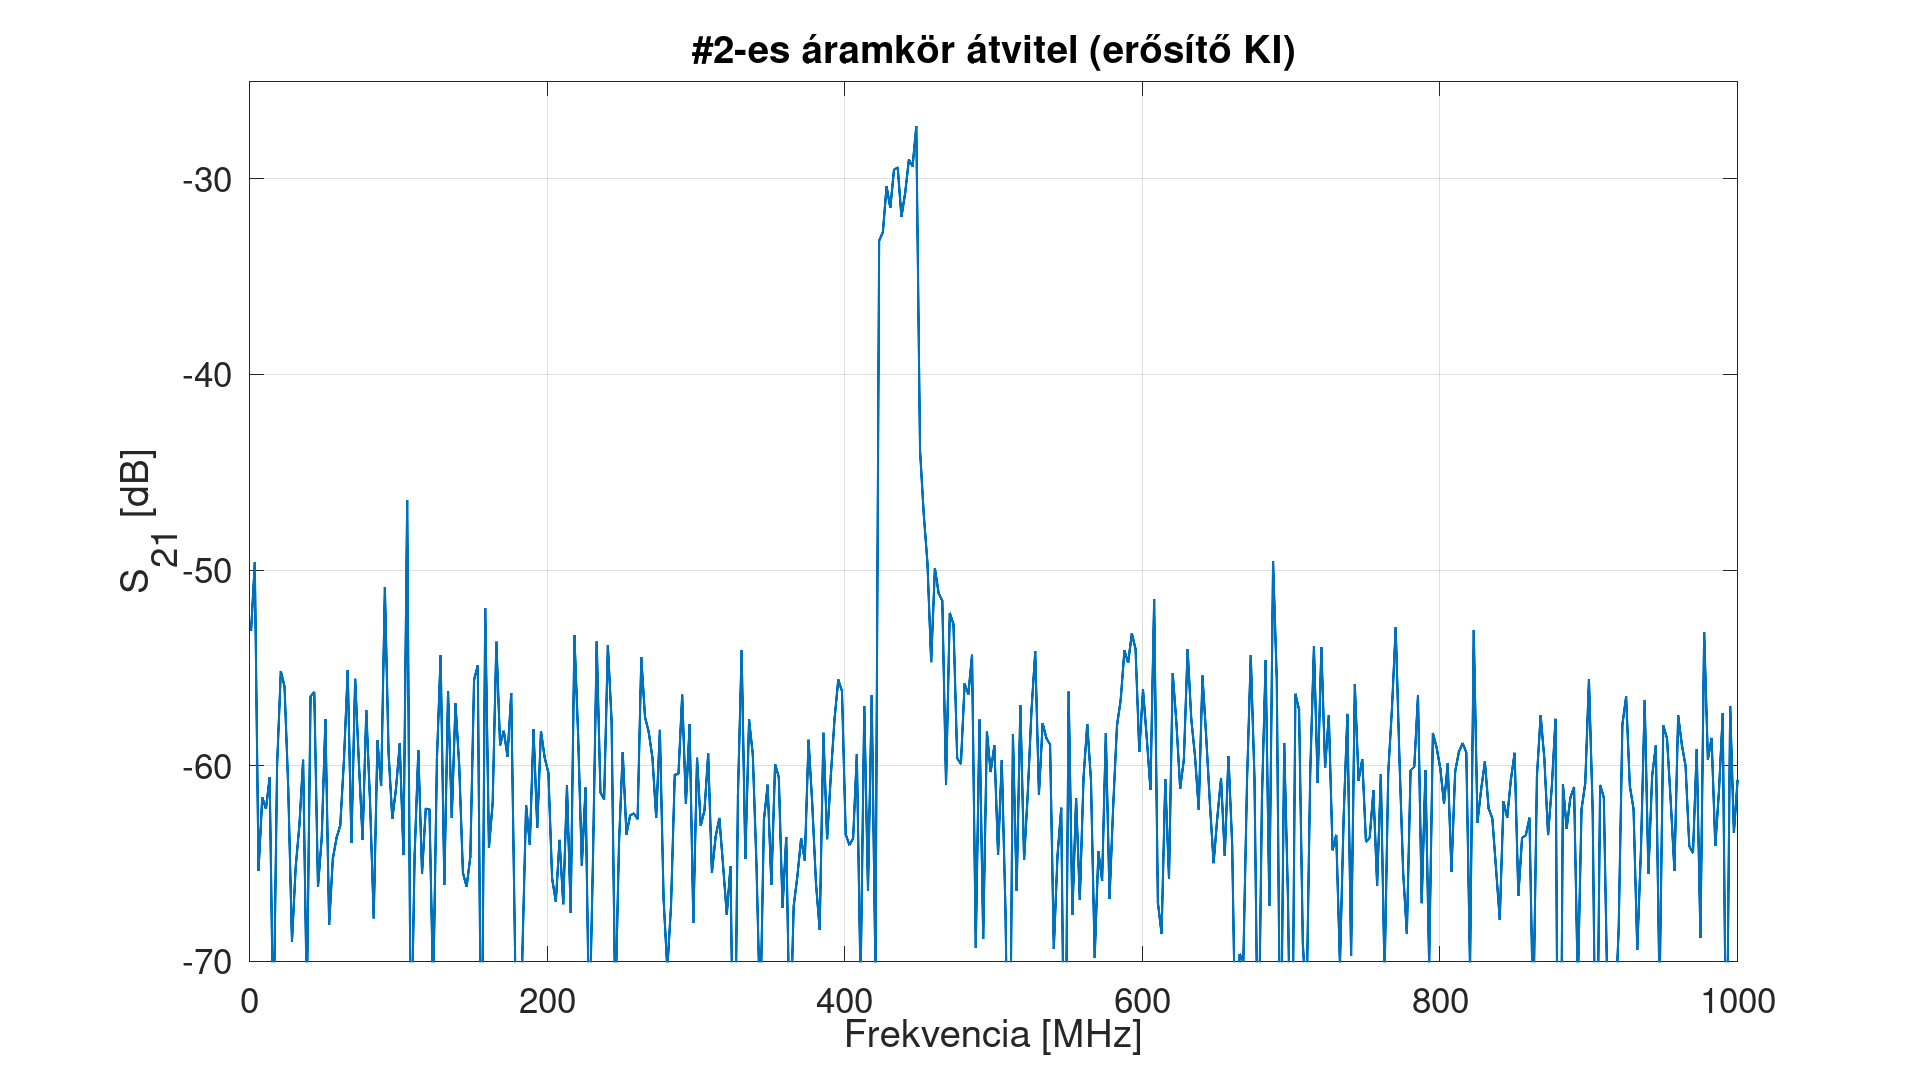
\includegraphics[keepaspectratio, width=\textwidth]{aramkor2_5.png}
	\caption{\#2-es erősítő 1\,MHz - 1\,GHz, erősítő KI}
	\label{fig:meres5}
\end{figure}

\begin{figure}[!ht]
	\centering
	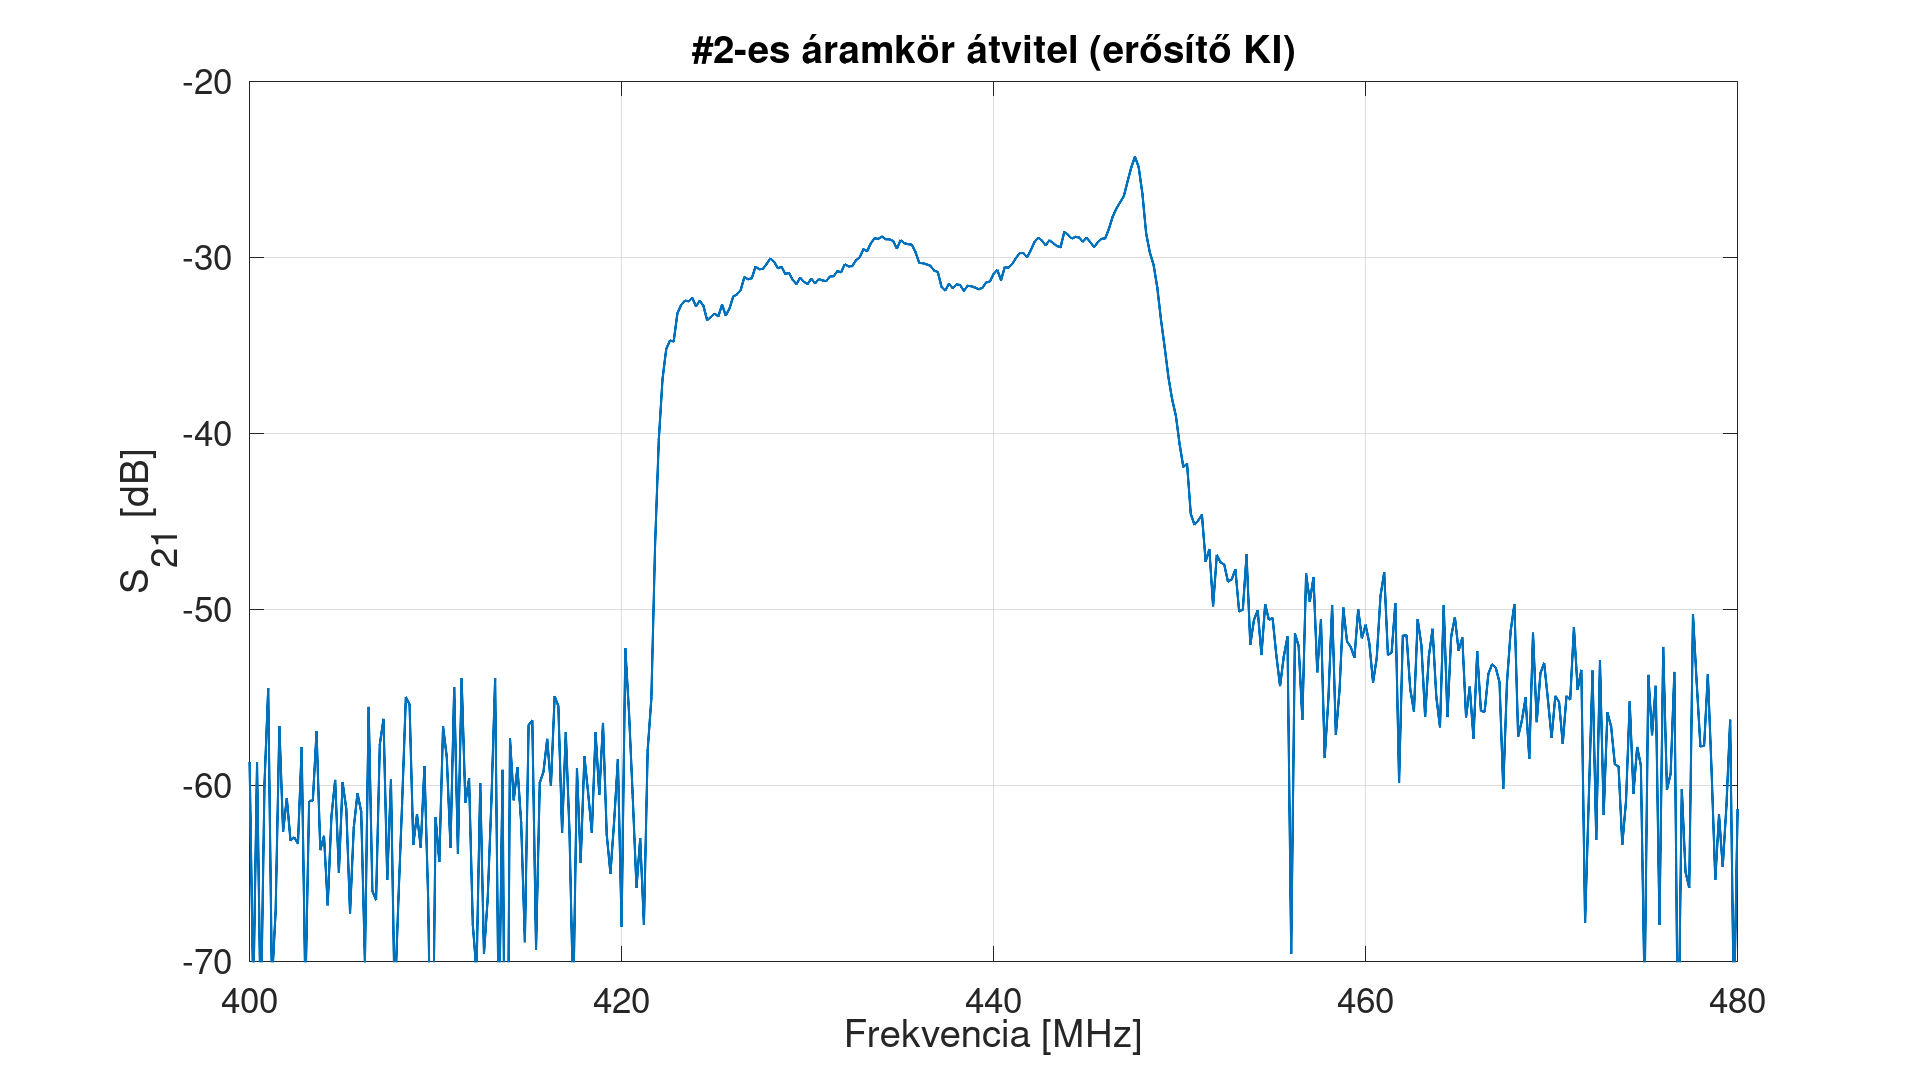
\includegraphics[keepaspectratio, width=\textwidth]{aramkor2_6.png}
	\caption{\#2-es erősítő 400\,MHz - 480\,MHz, erősítő KI}
	\label{fig:meres6}
\end{figure}

\begin{figure}[!ht]
	\centering
	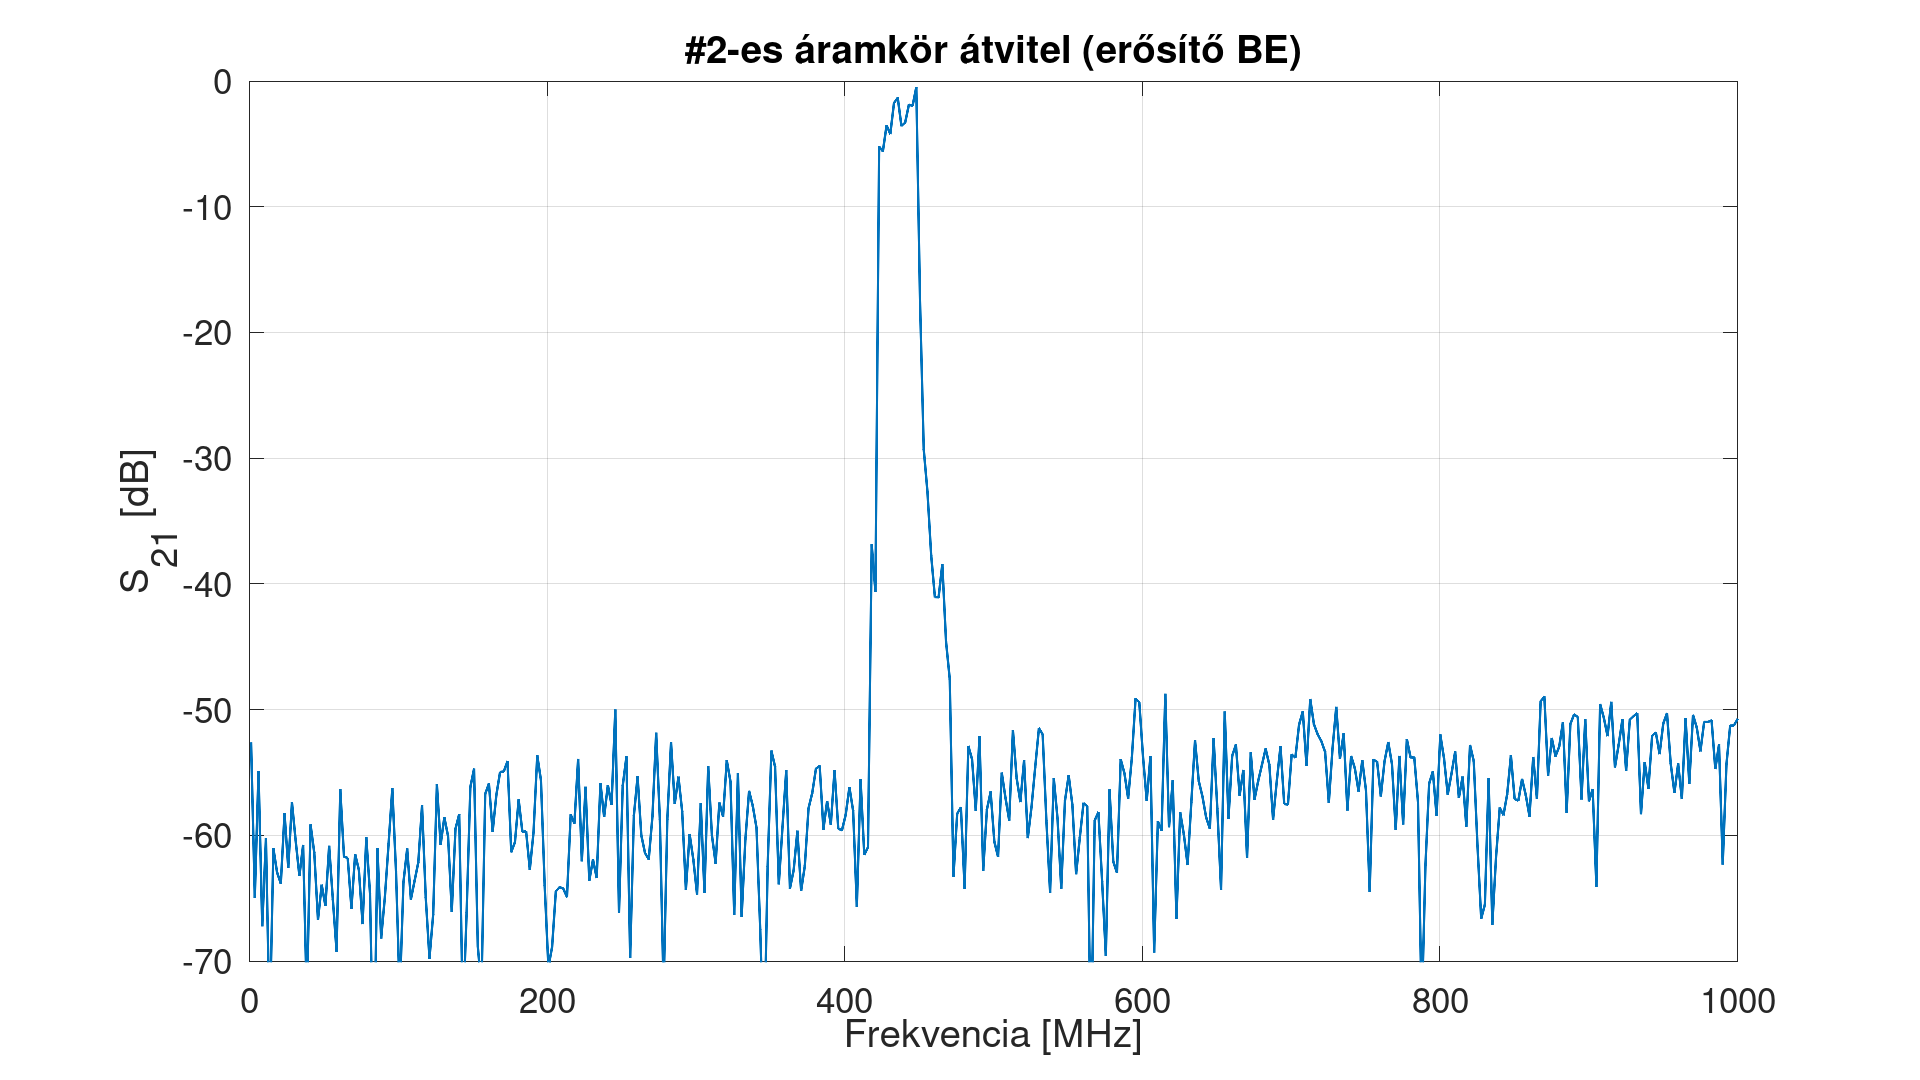
\includegraphics[keepaspectratio, width=\textwidth]{aramkor2_7.png}
	\caption{\#2-es erősítő 1\,MHz - 1\,GHz, erősítő BE}
	\label{fig:meres7}
\end{figure}

\begin{figure}[!ht]
	\centering
	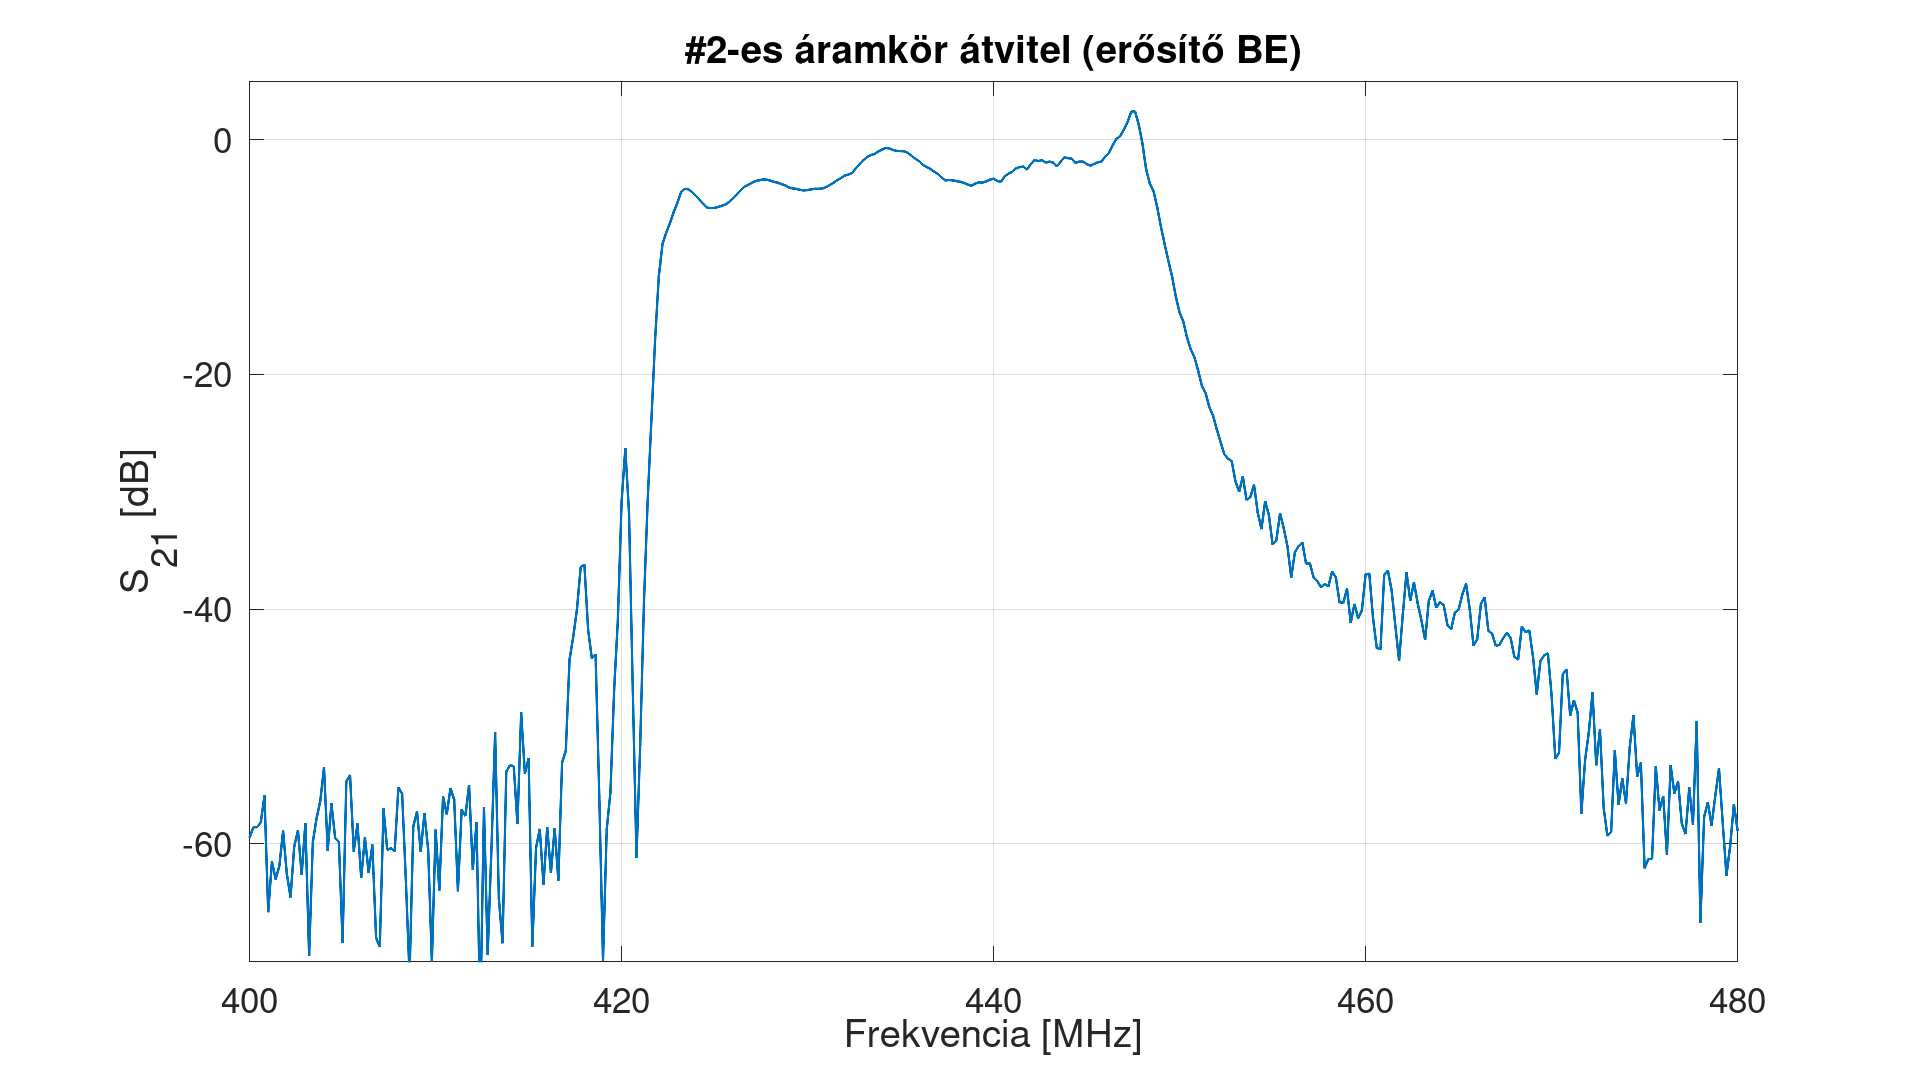
\includegraphics[keepaspectratio, width=\textwidth]{aramkor2_8.png}
	\caption{\#2-es erősítő 400\,MHz - 480\,MHz, erősítő BE}
	\label{fig:meres8}
\end{figure}

\begin{figure}[!ht]
	\centering
	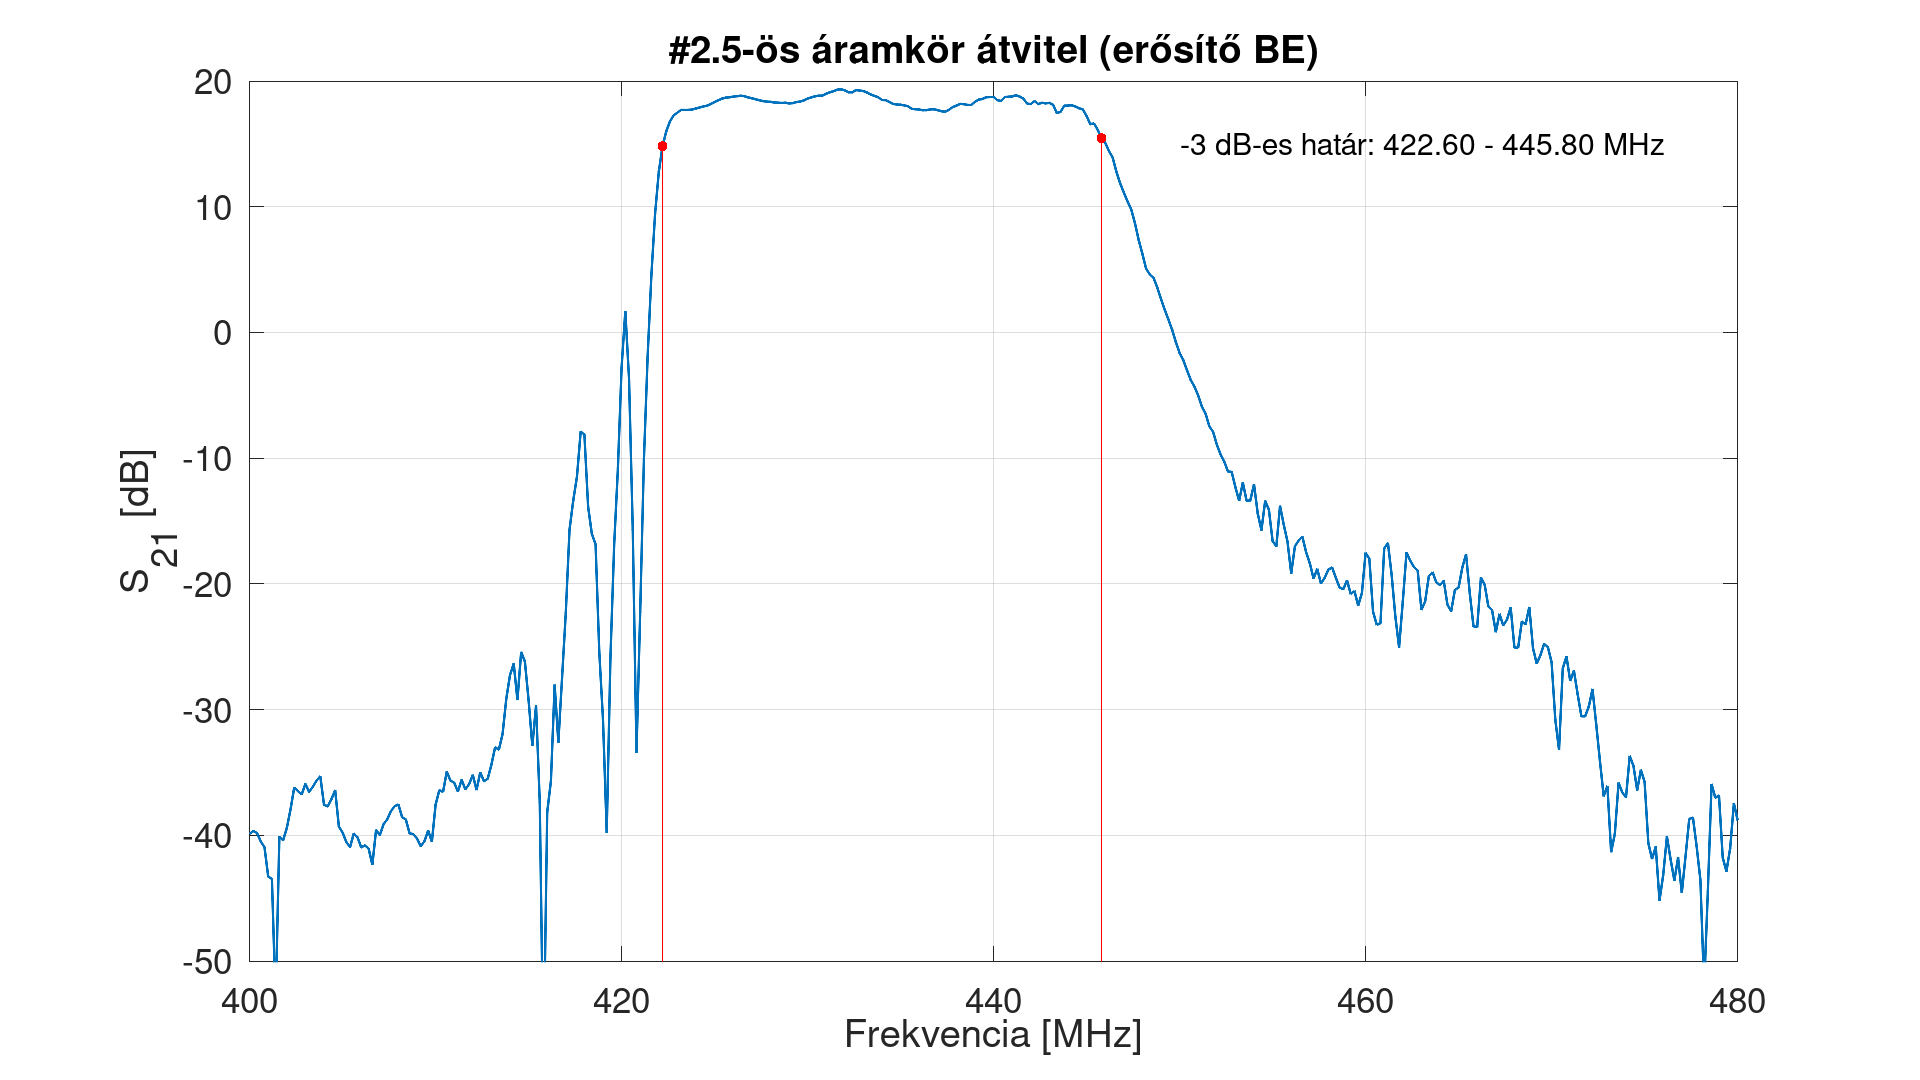
\includegraphics[keepaspectratio, width=\textwidth]{aramkor2_14.png}
	\caption{\#2.5-ös erősítő 400\,MHz - 480\,MHz, erősítő BE}
	\label{fig:meres14}
\end{figure}



\begin{figure}[!ht]
	\centering
	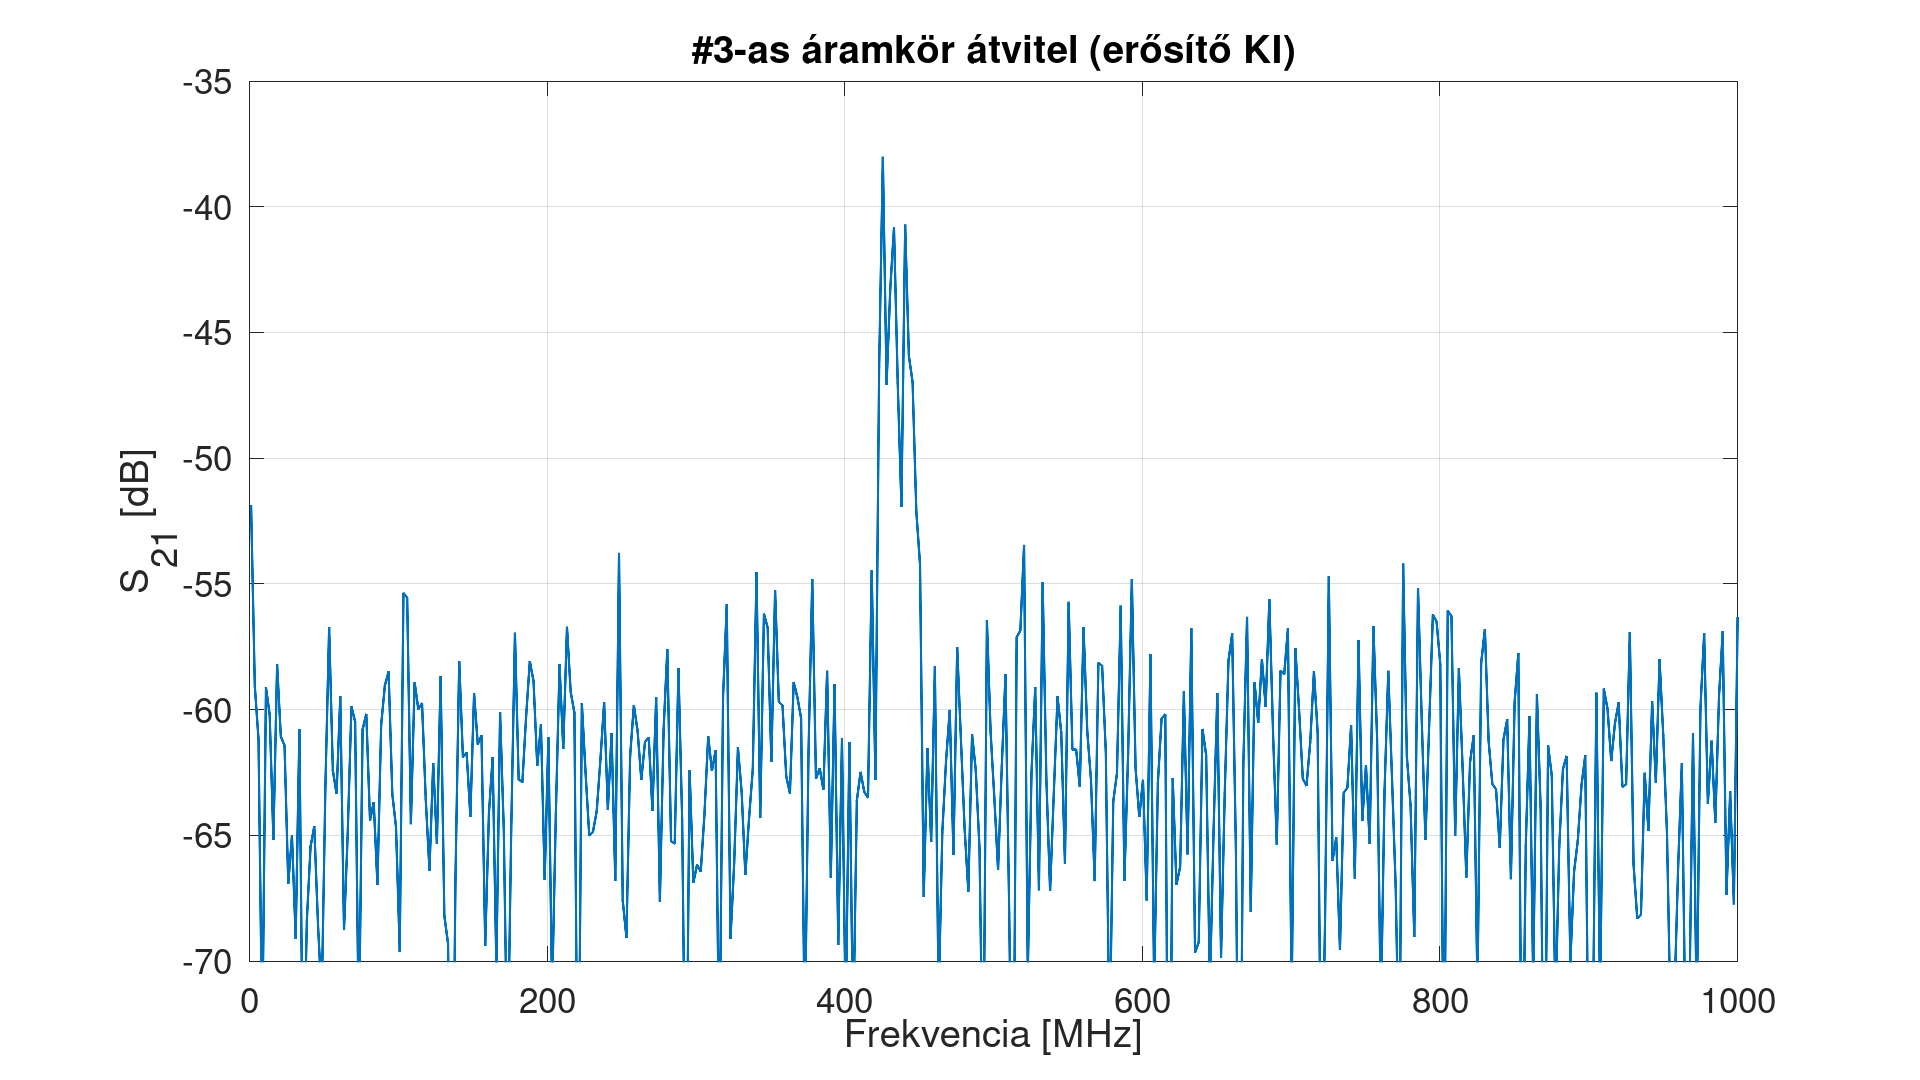
\includegraphics[keepaspectratio, width=\textwidth]{aramkor3_9.png}
	\caption{\#3-as erősítő 1\,MHz - 1\,GHz, erősítő KI}
	\label{fig:meres9}
\end{figure}

\begin{figure}[!ht]
	\centering
	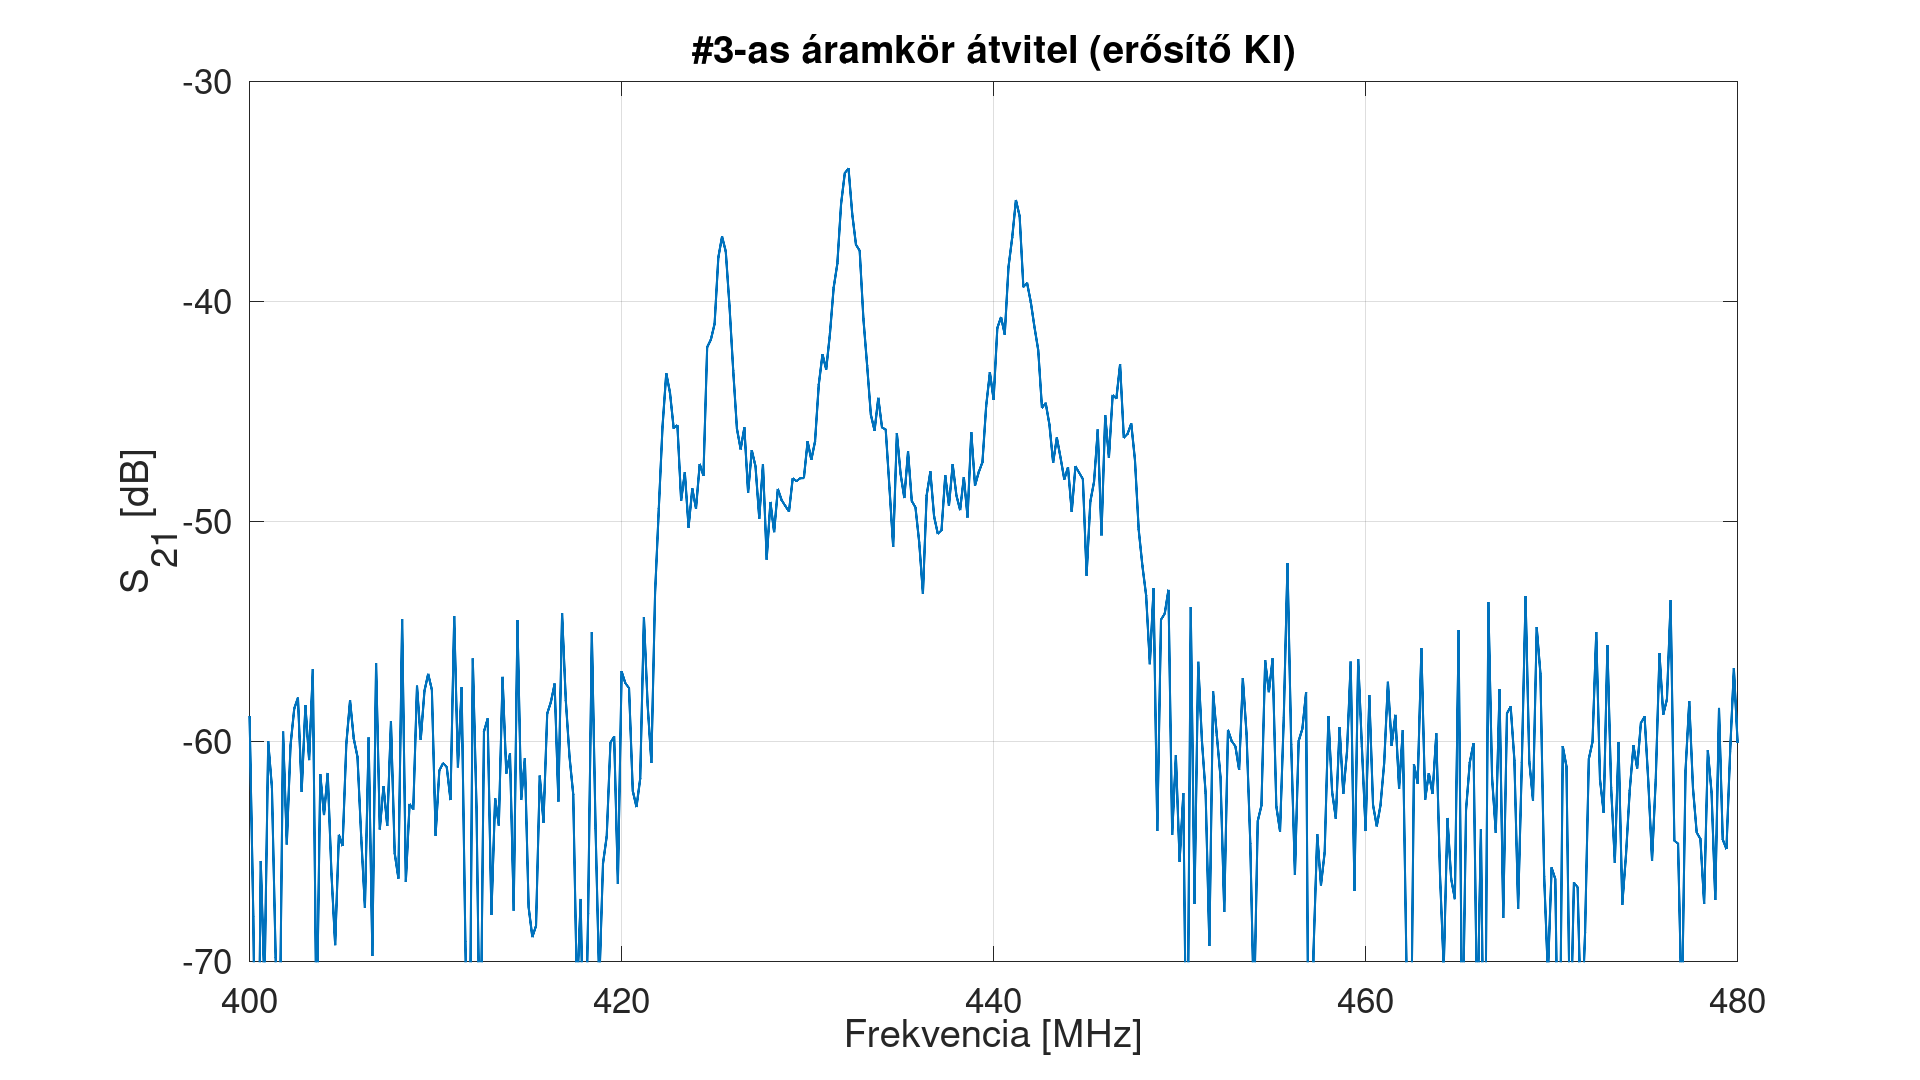
\includegraphics[keepaspectratio, width=\textwidth]{aramkor3_10.png}
	\caption{\#3-as erősítő 400\,MHz - 480\,MHz, erősítő KI}
	\label{fig:meres10}
\end{figure}

\begin{figure}[!ht]
	\centering
	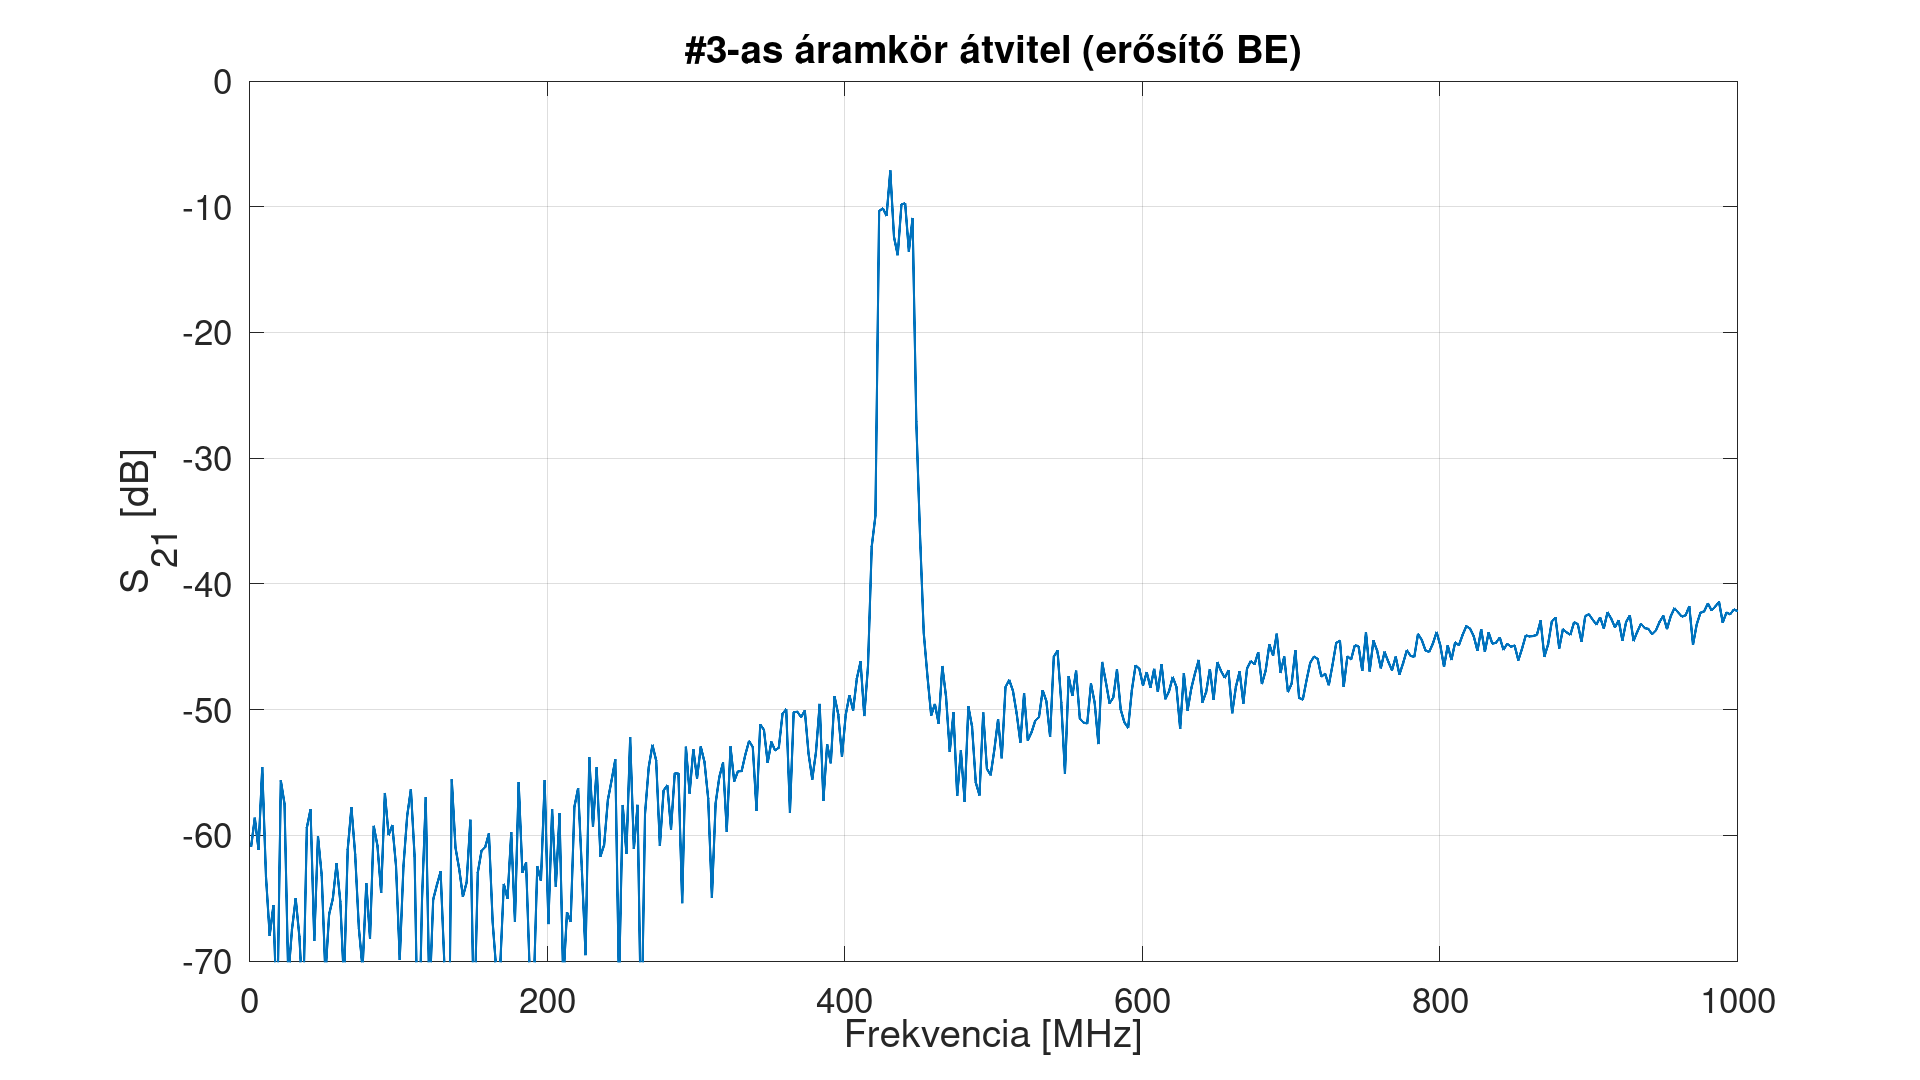
\includegraphics[keepaspectratio, width=\textwidth]{aramkor3_11.png}
	\caption{\#3-as erősítő 1\,MHz - 1\,GHz, erősítő BE}
	\label{fig:meres11}
\end{figure}

\begin{figure}[!ht]
	\centering
	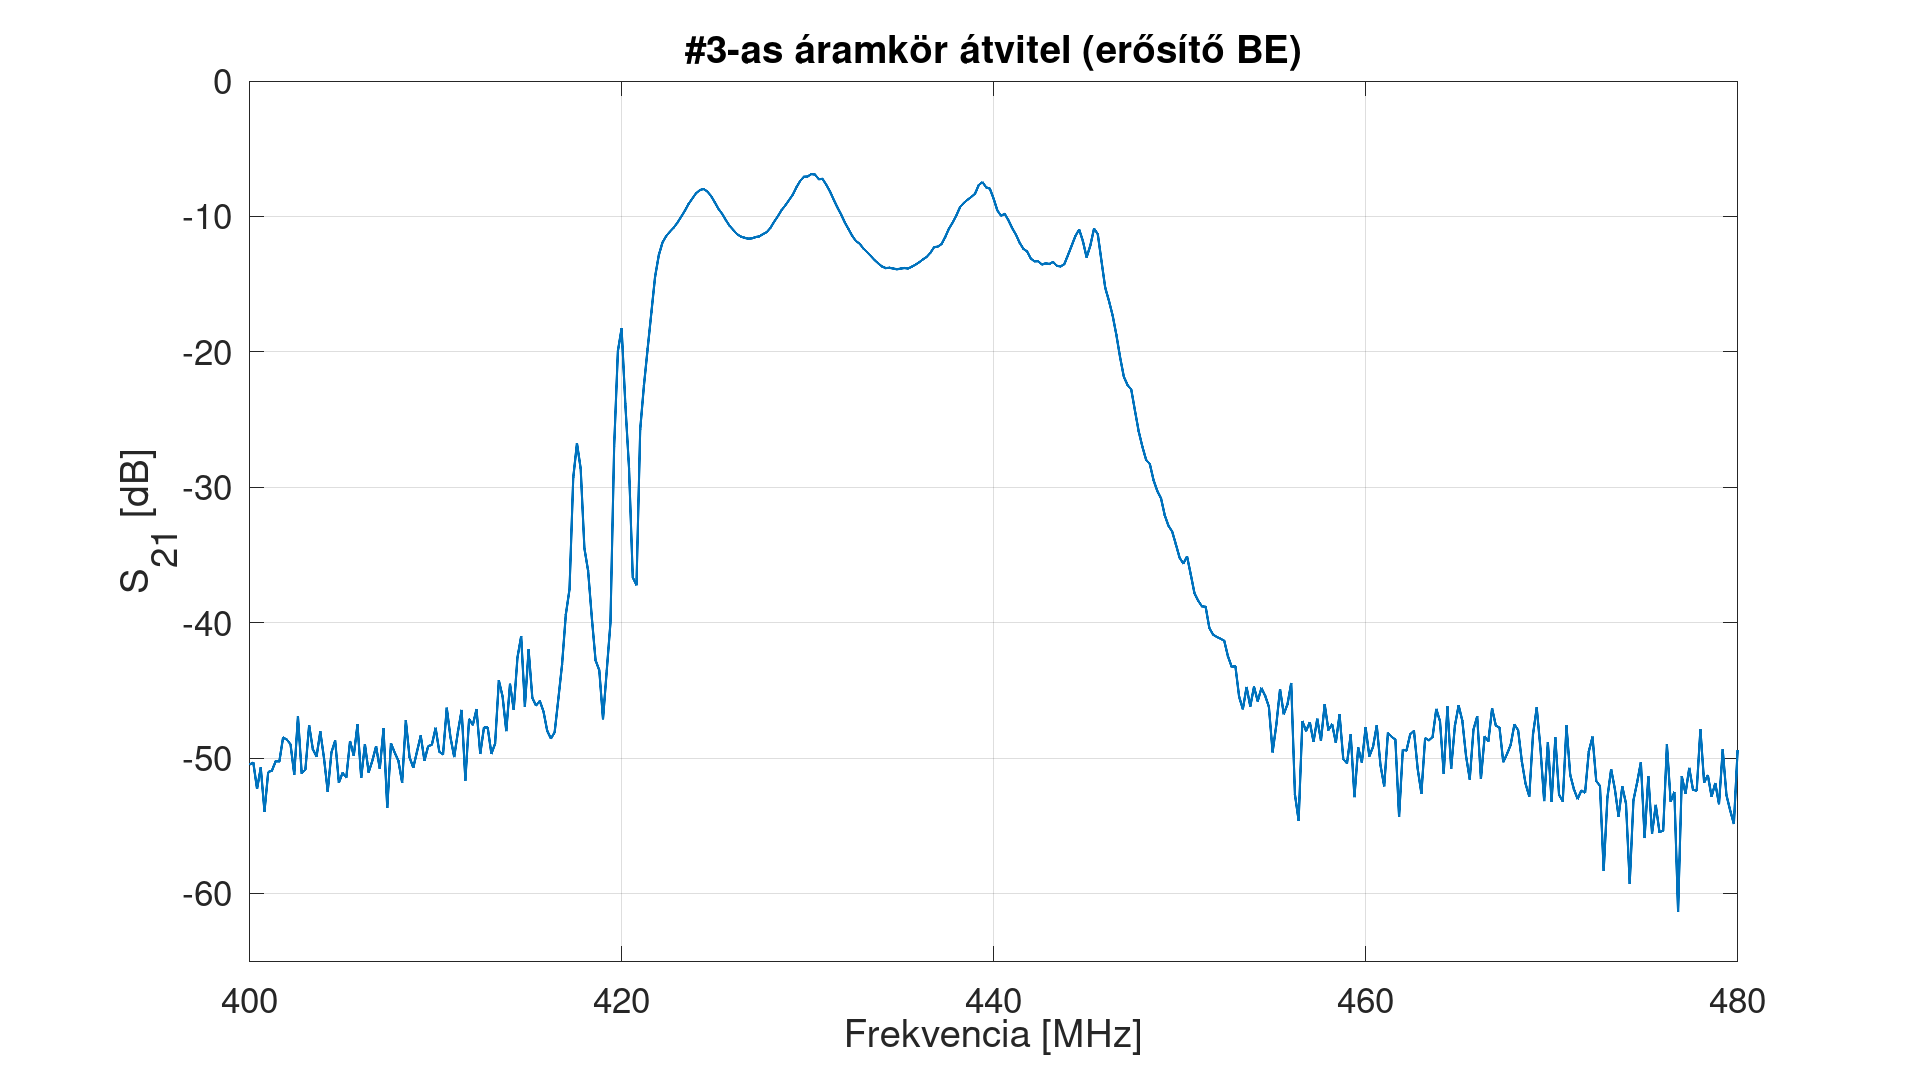
\includegraphics[keepaspectratio, width=\textwidth]{aramkor3_12.png}
	\caption{\#3-as erősítő 400\,MHz - 480\,MHz, erősítő BE}
	\label{fig:meres12}
\end{figure}



\begin{figure}[!ht]
	\centering
	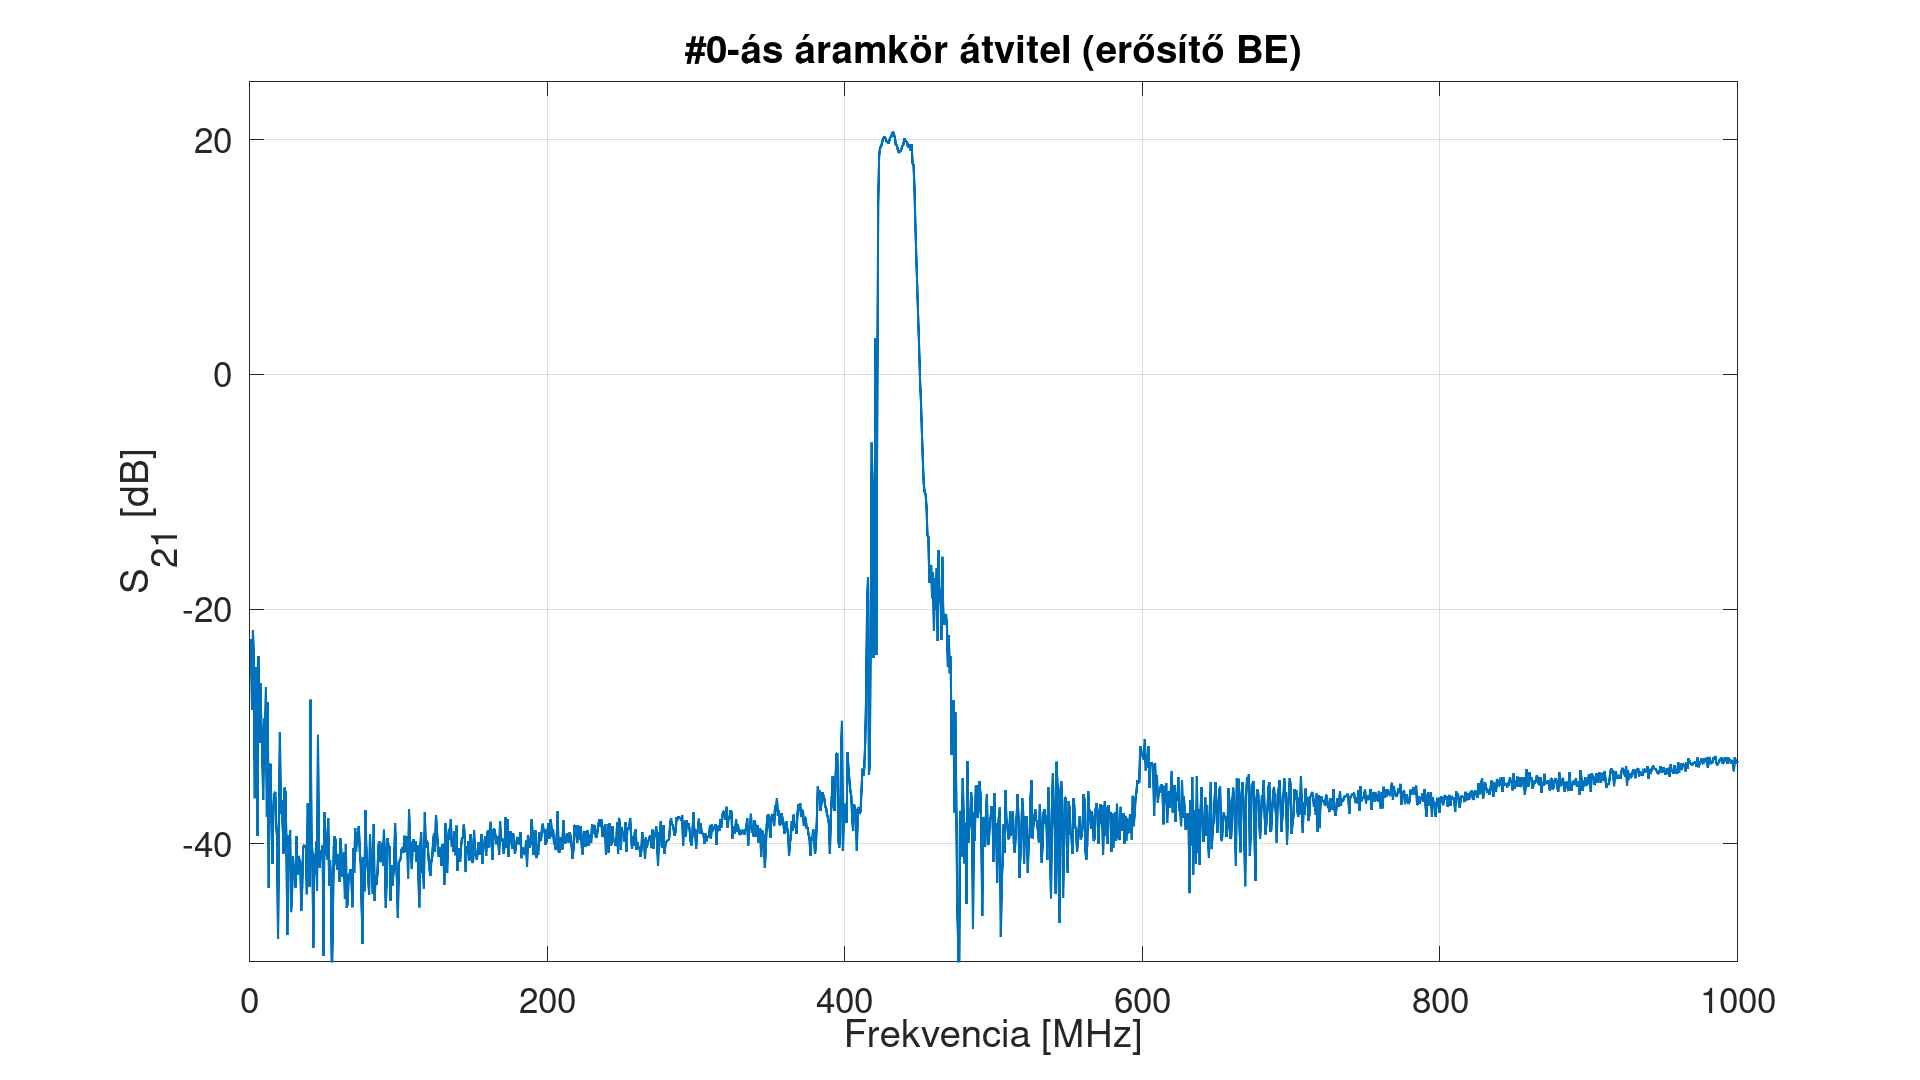
\includegraphics[keepaspectratio, width=\textwidth]{aramkor0_01.png}
	\caption{\#0-ás erősítő 1\,MHz - 1\,GHz, erősítő BE}
	\label{fig:meres01}
\end{figure}

\begin{figure}[!ht]
	\centering
	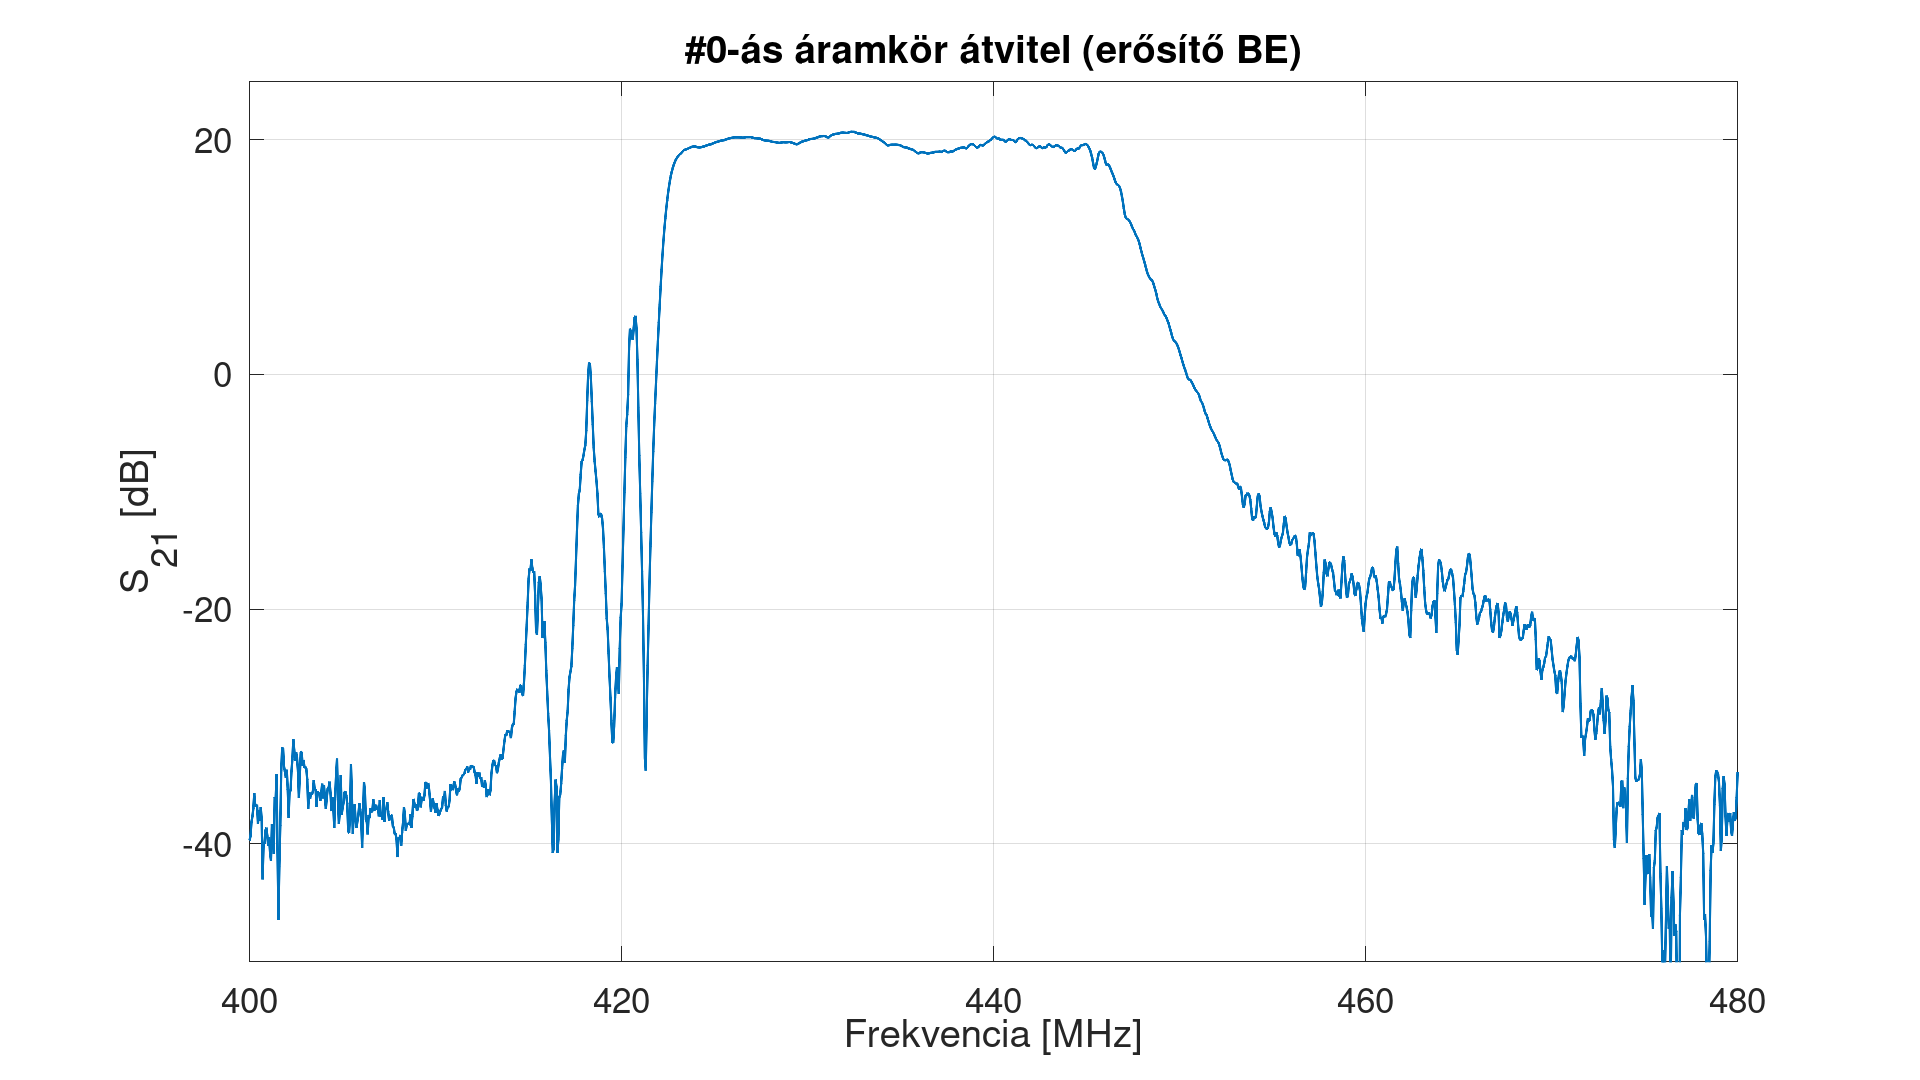
\includegraphics[keepaspectratio, width=\textwidth]{aramkor0_02.png}
	\caption{\#0-ás erősítő 400\,MHz - 480\,MHz, erősítő BE}
	\label{fig:meres02}
\end{figure}



\begin{figure}[!ht]
	\centering
	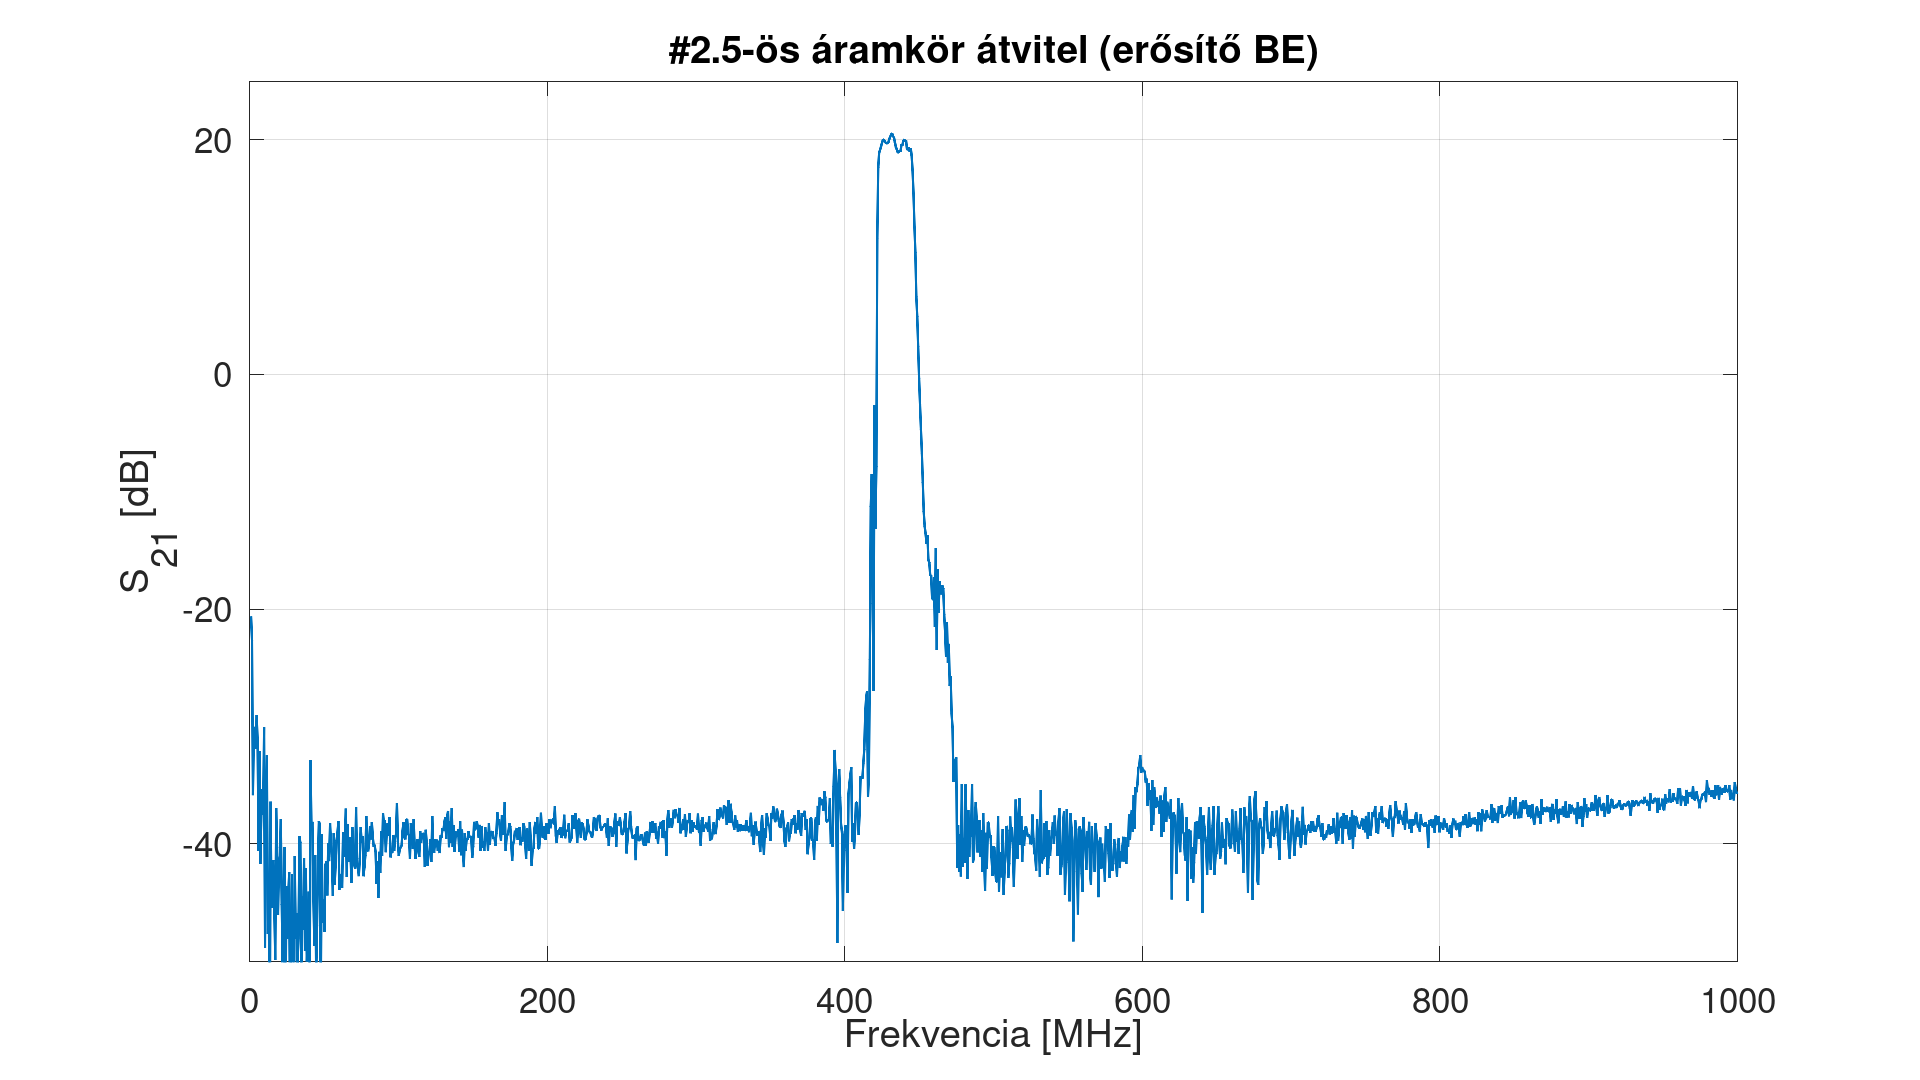
\includegraphics[keepaspectratio, width=\textwidth]{aramkor2_21.png}
	\caption{\#2.5-ös erősítő 1\,MHz - 1\,GHz, erősítő BE}
	\label{fig:meres21}
\end{figure}

\begin{figure}[!ht]
	\centering
	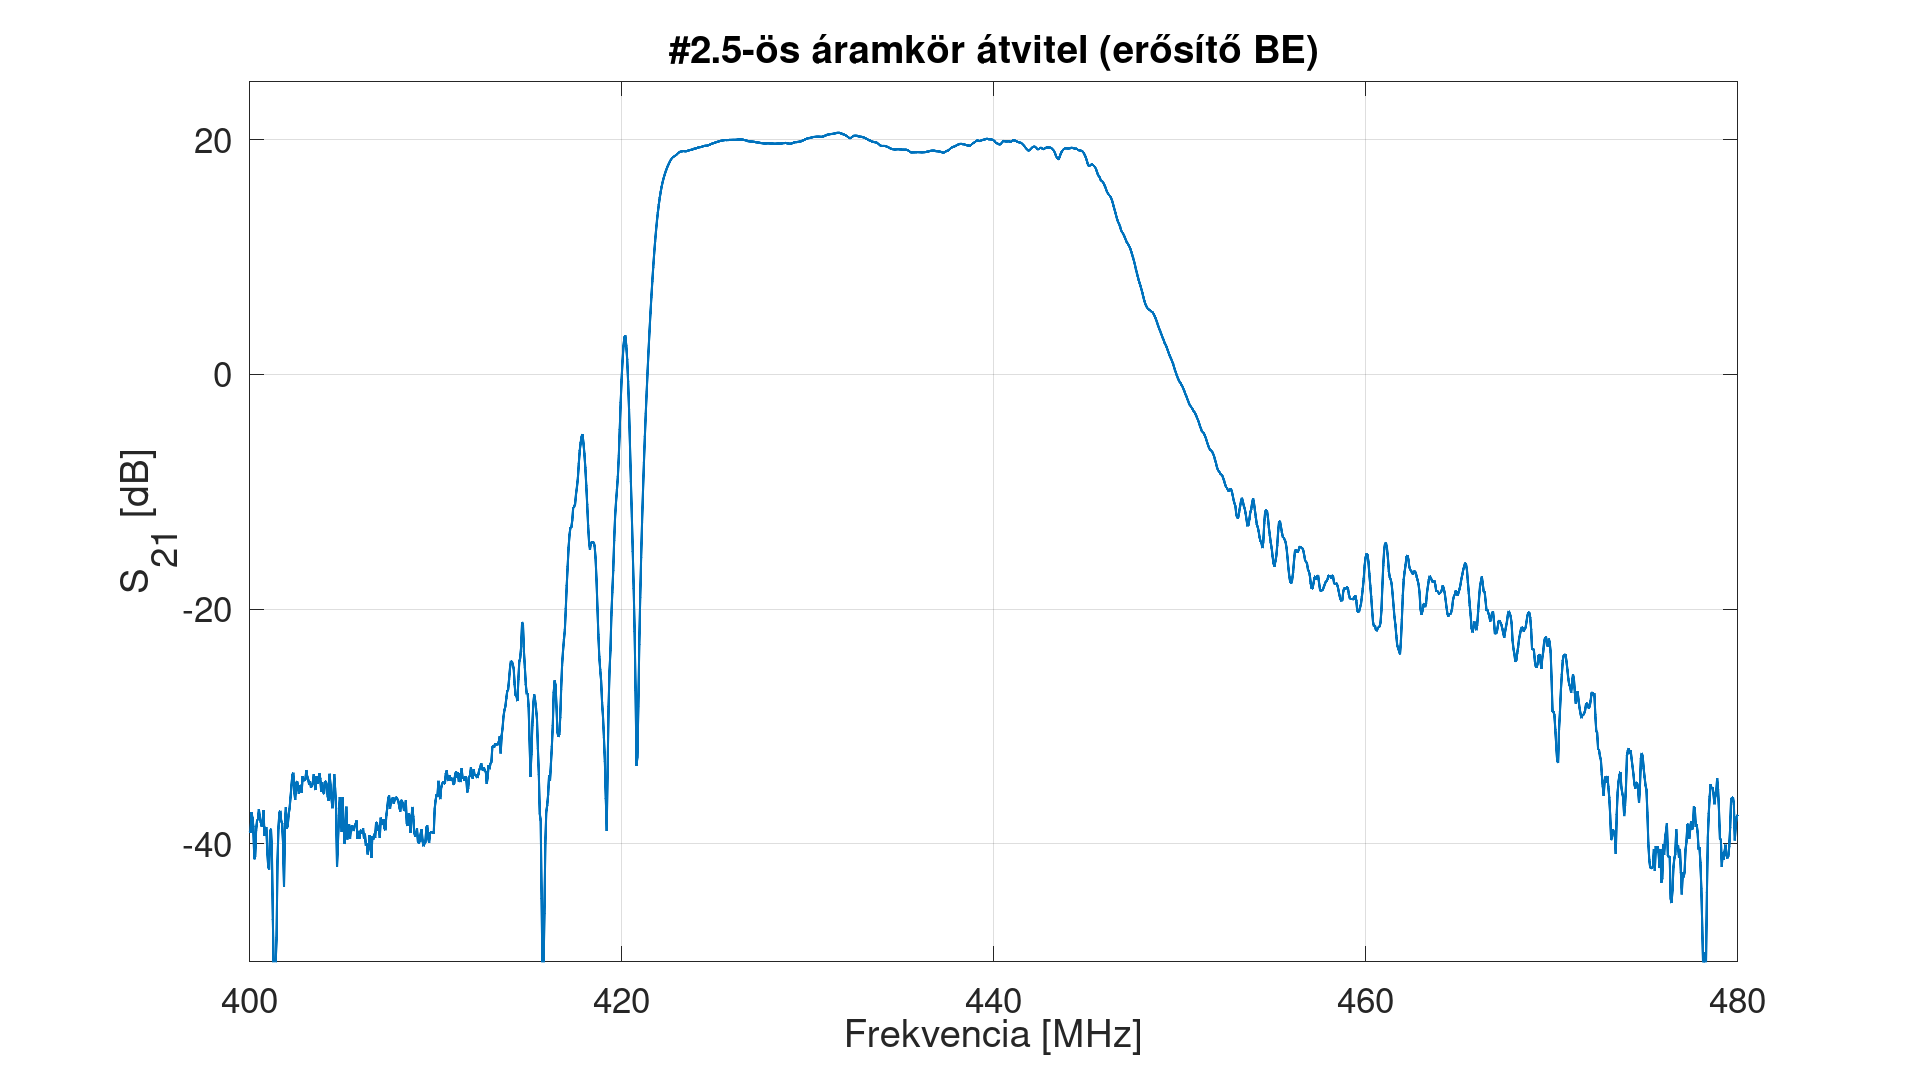
\includegraphics[keepaspectratio, width=\textwidth]{aramkor2_22.png}
	\caption{\#2.5-ös erősítő 400\,MHz - 480\,MHz, erősítő BE}
	\label{fig:meres22}
\end{figure}



\begin{figure}[!ht]
	\centering
	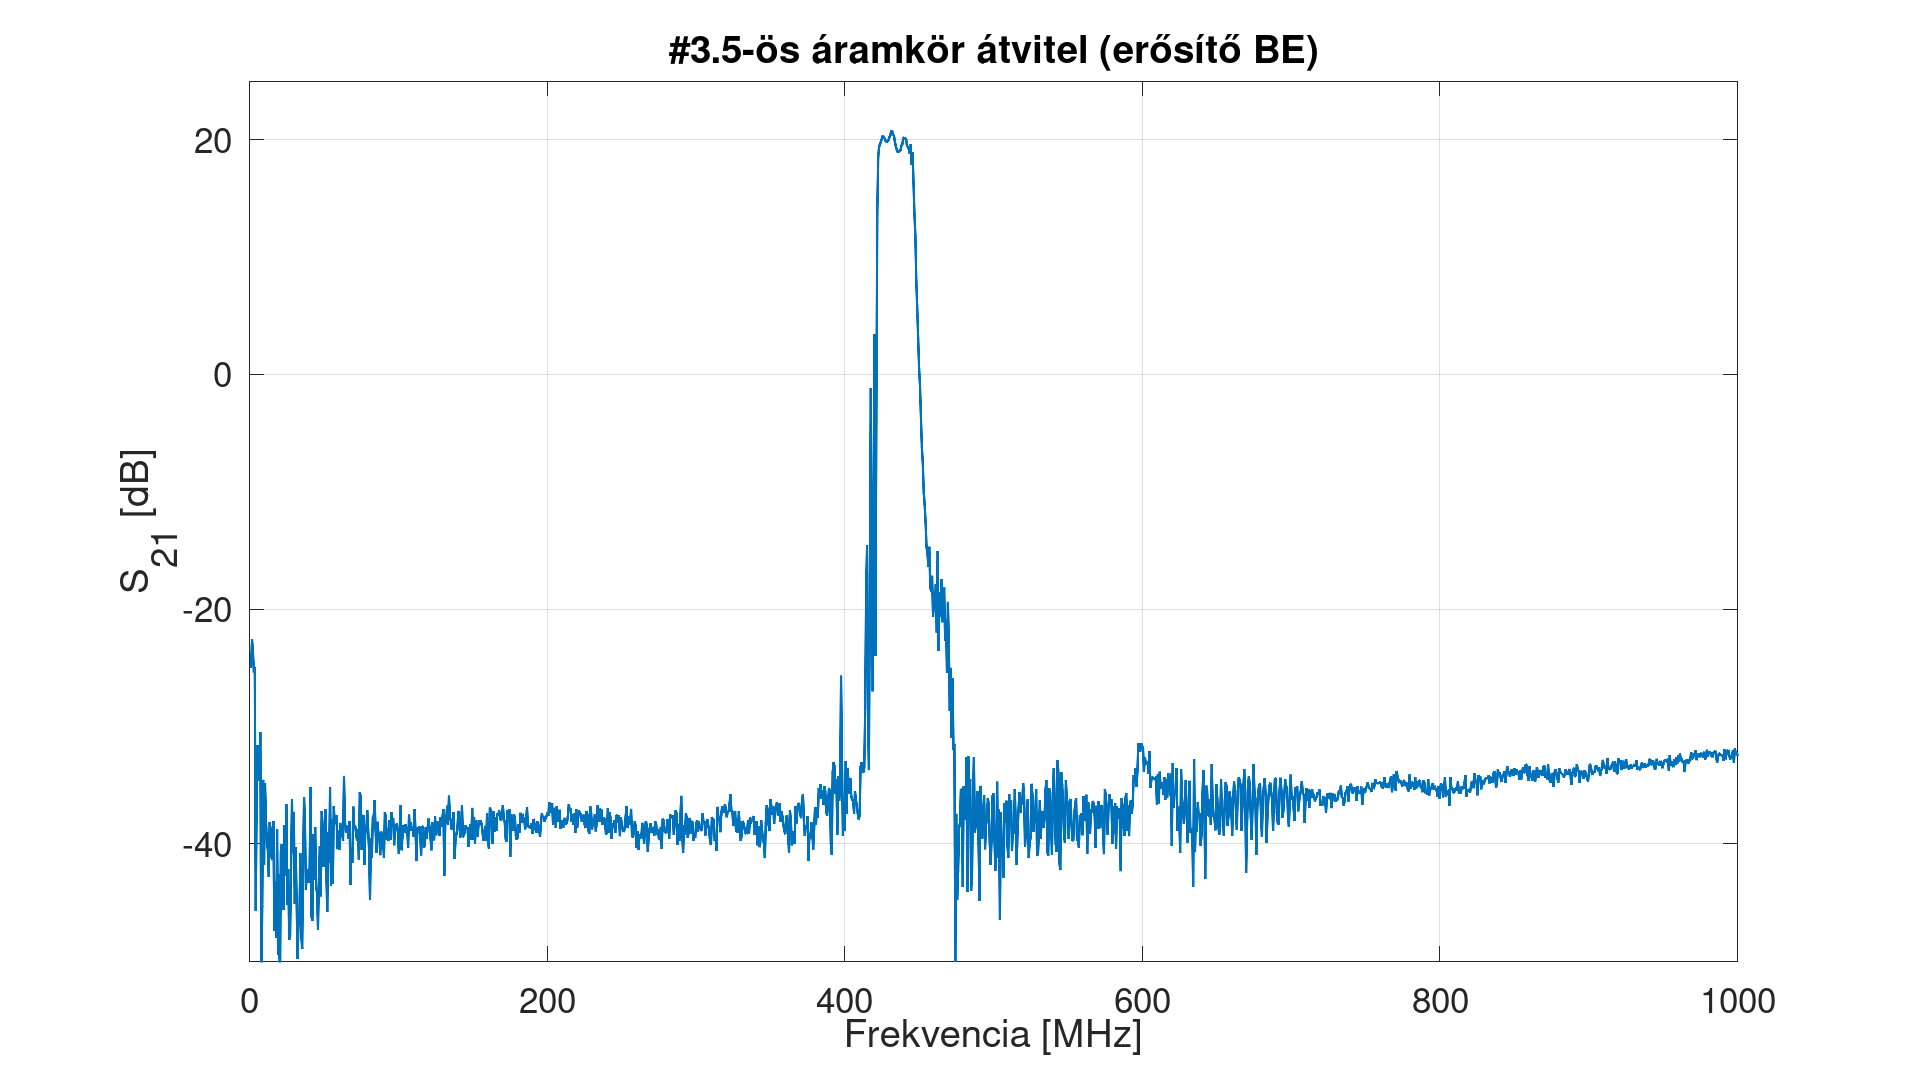
\includegraphics[keepaspectratio, width=\textwidth]{aramkor3_31.png}
	\caption{\#3.5-ös erősítő 1\,MHz - 1\,GHz, erősítő BE}
	\label{fig:meres31}
\end{figure}

\begin{figure}[!ht]
	\centering
	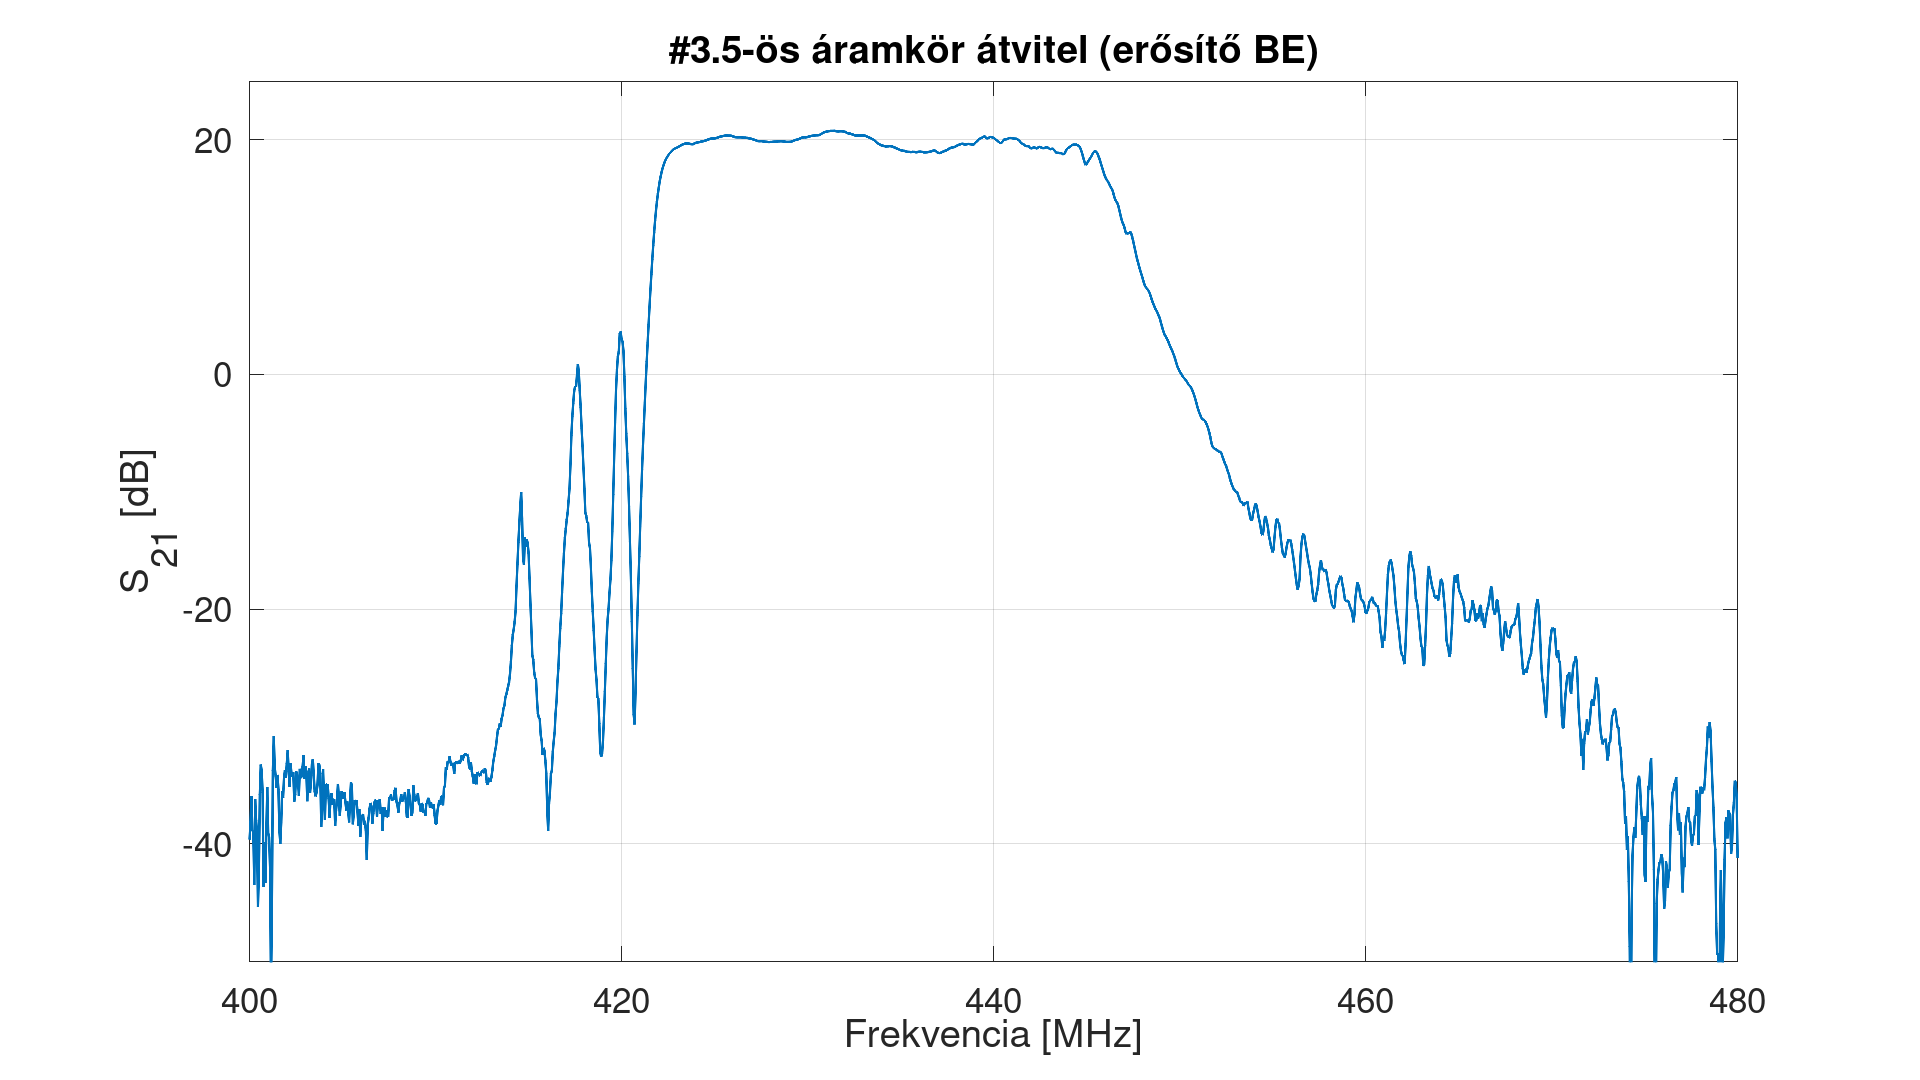
\includegraphics[keepaspectratio, width=\textwidth]{aramkor3_32.png}
	\caption{\#3.5-ös erősítő 400\,MHz - 480\,MHz, erősítő BE}
	\label{fig:meres32}
\end{figure}



\begin{figure}[!ht]
	\centering
	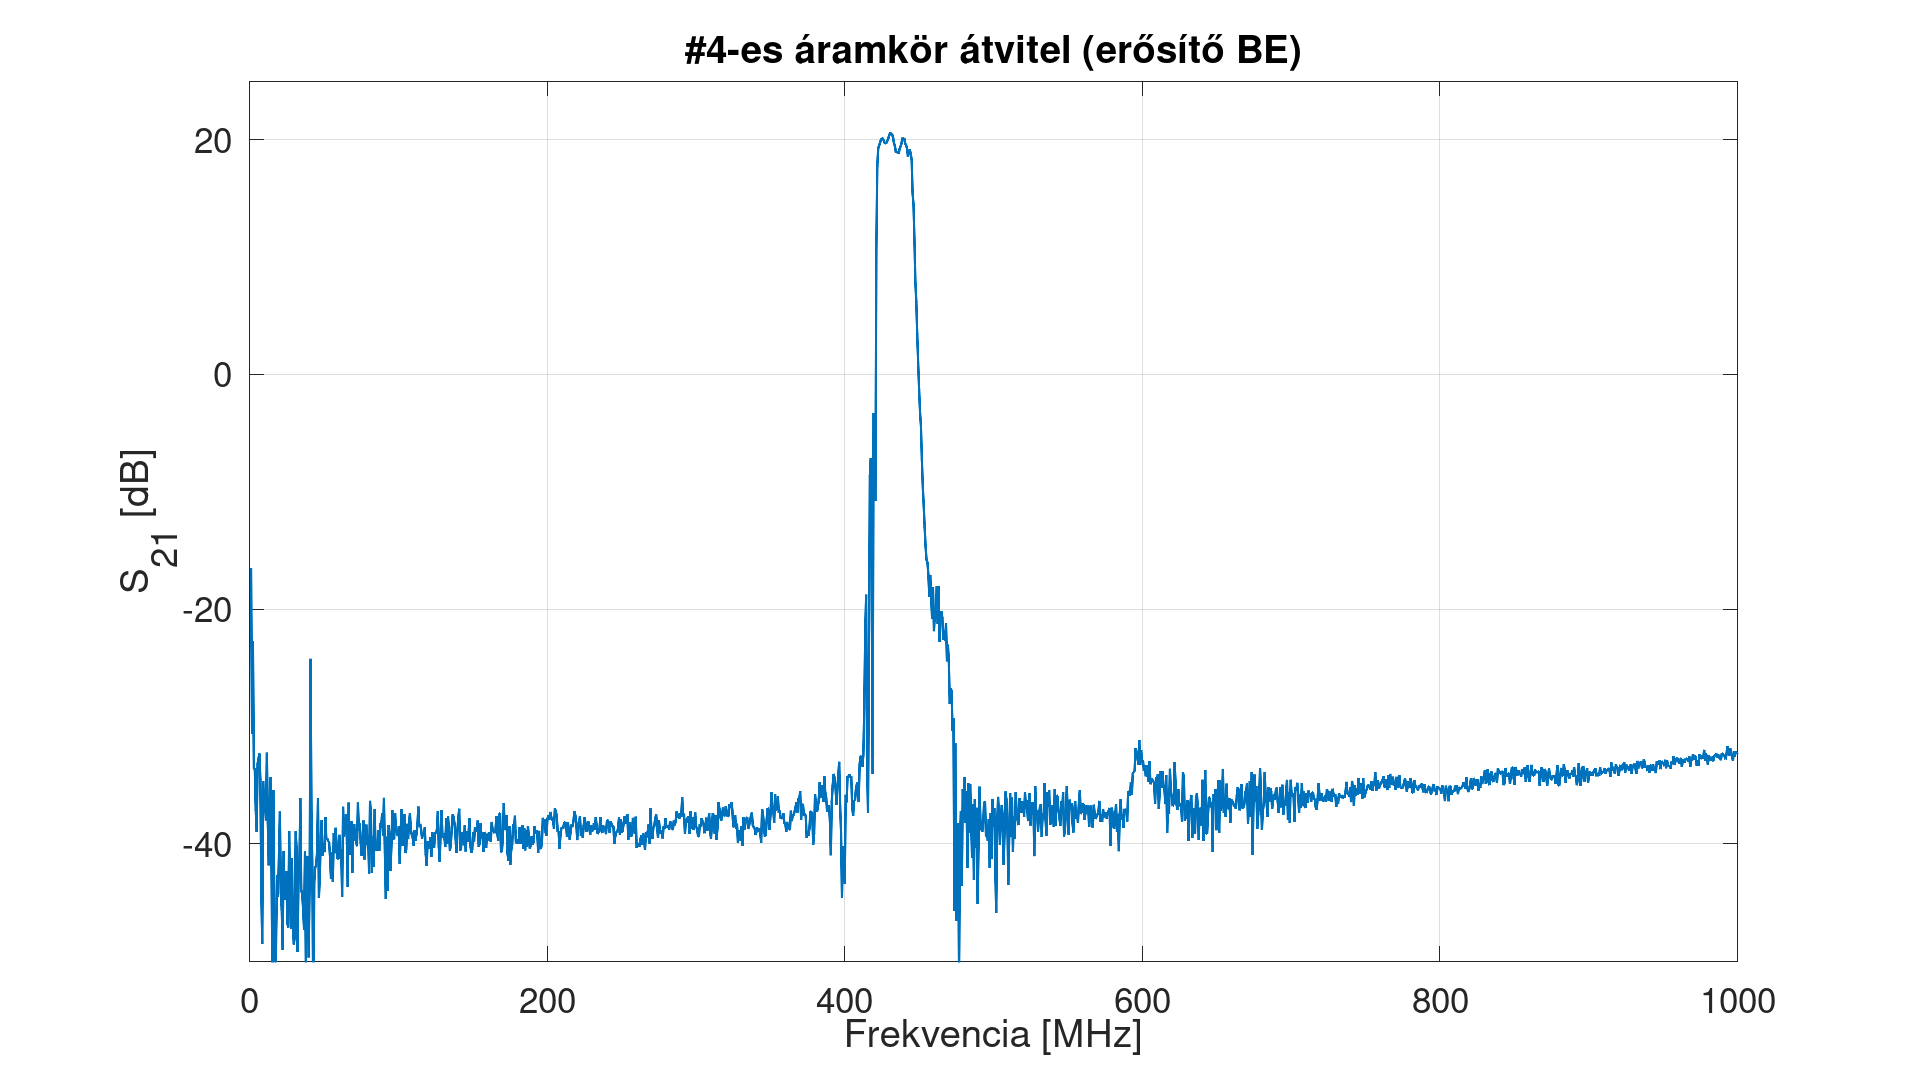
\includegraphics[keepaspectratio, width=\textwidth]{aramkor4_41.png}
	\caption{\#4-es erősítő 1\,MHz - 1\,GHz, erősítő BE}
	\label{fig:meres41}
\end{figure}

\begin{figure}[!ht]
	\centering
	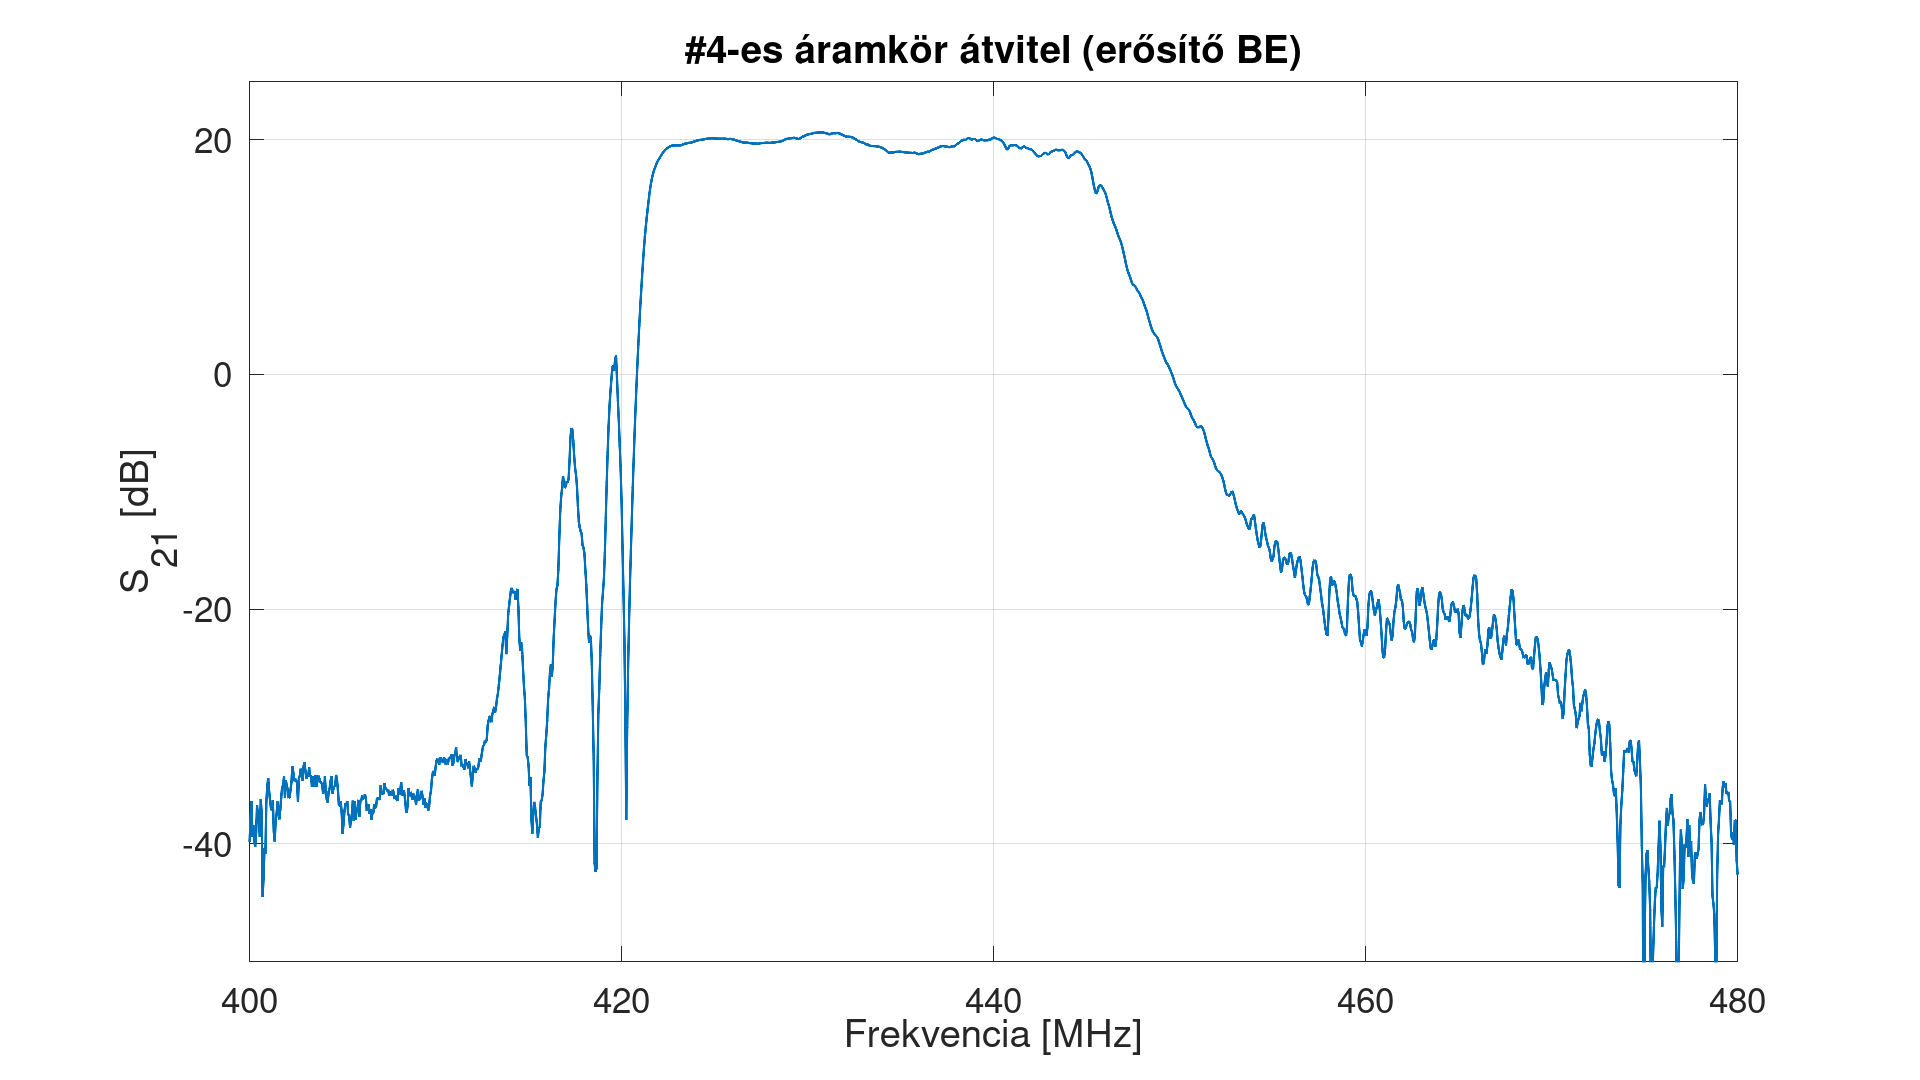
\includegraphics[keepaspectratio, width=\textwidth]{aramkor4_42.png}
	\caption{\#4-es erősítő 400\,MHz - 480\,MHz, erősítő BE}
	\label{fig:meres42}
\end{figure}



\begin{figure}[!ht]
	\centering
	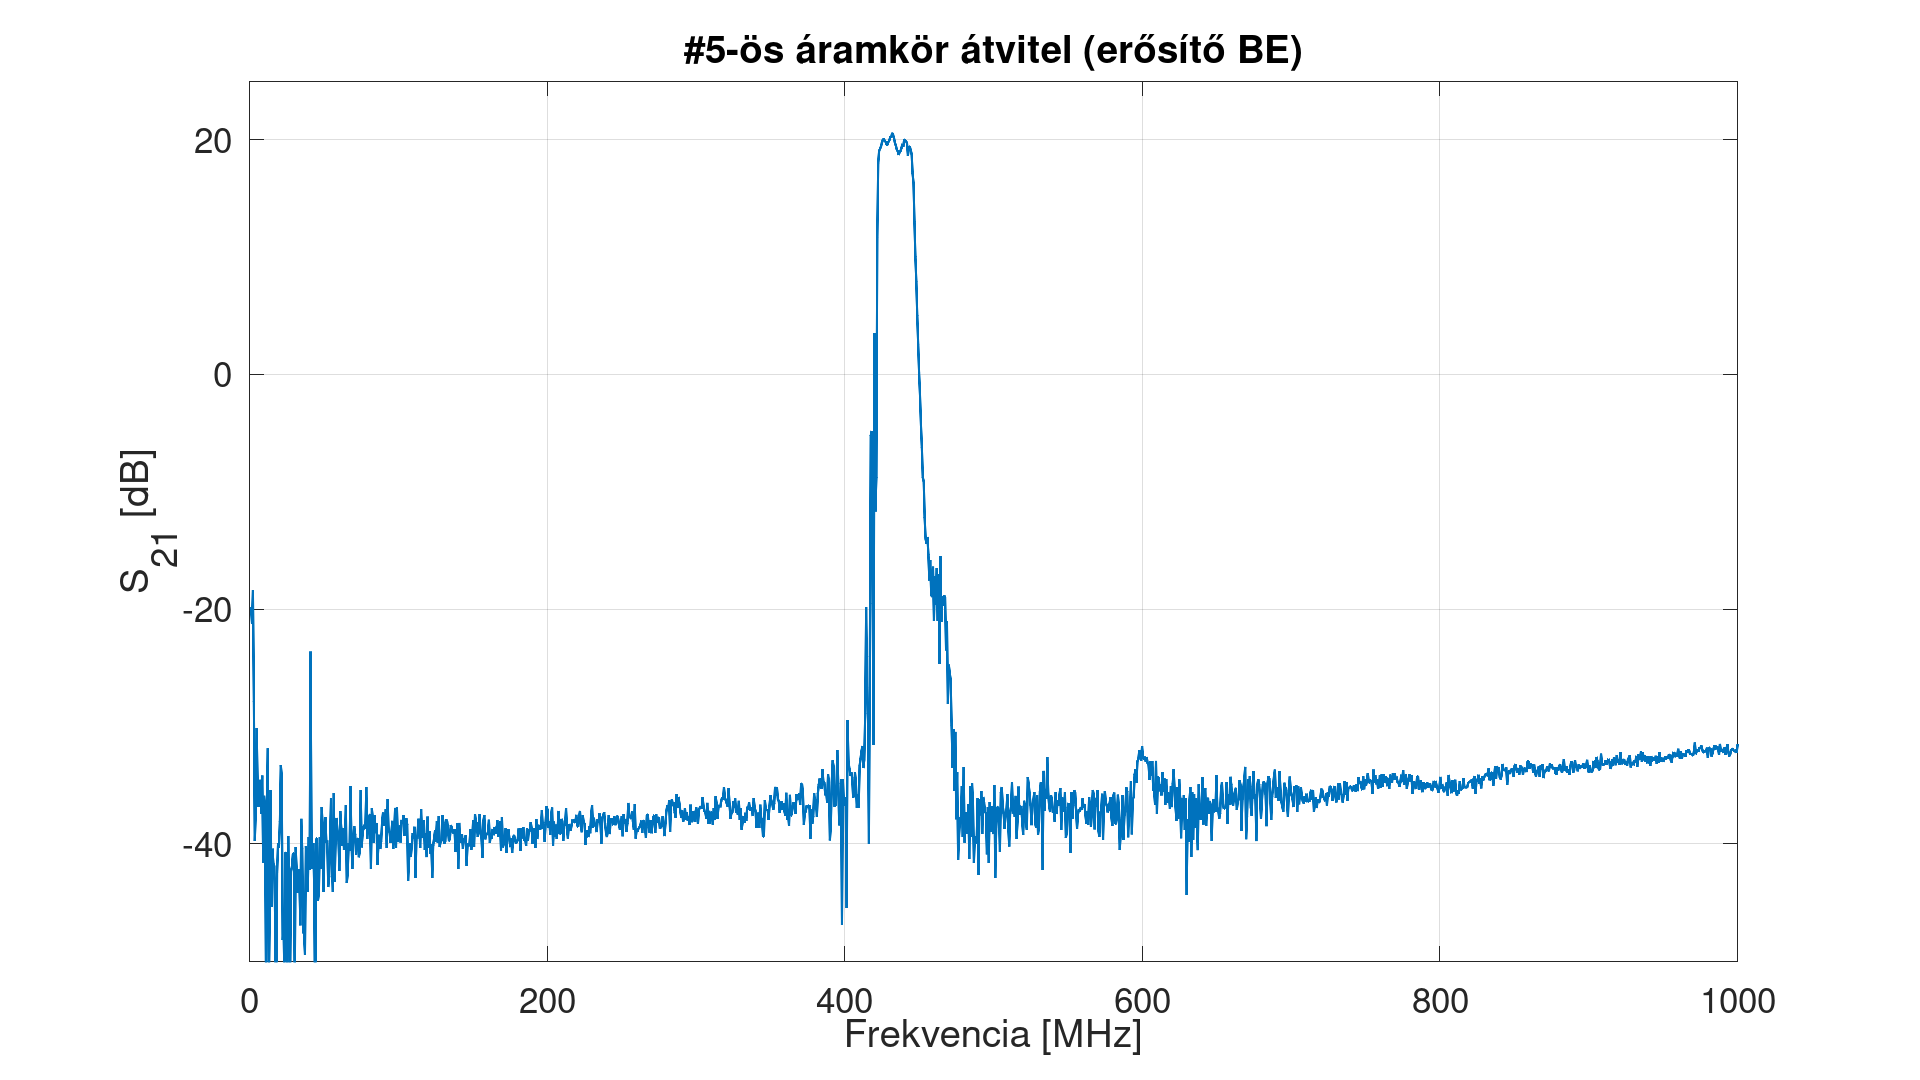
\includegraphics[keepaspectratio, width=\textwidth]{aramkor5_51.png}
	\caption{\#5-ös erősítő 1\,MHz - 1\,GHz, erősítő BE}
	\label{fig:meres51}
\end{figure}

\begin{figure}[!ht]
	\centering
	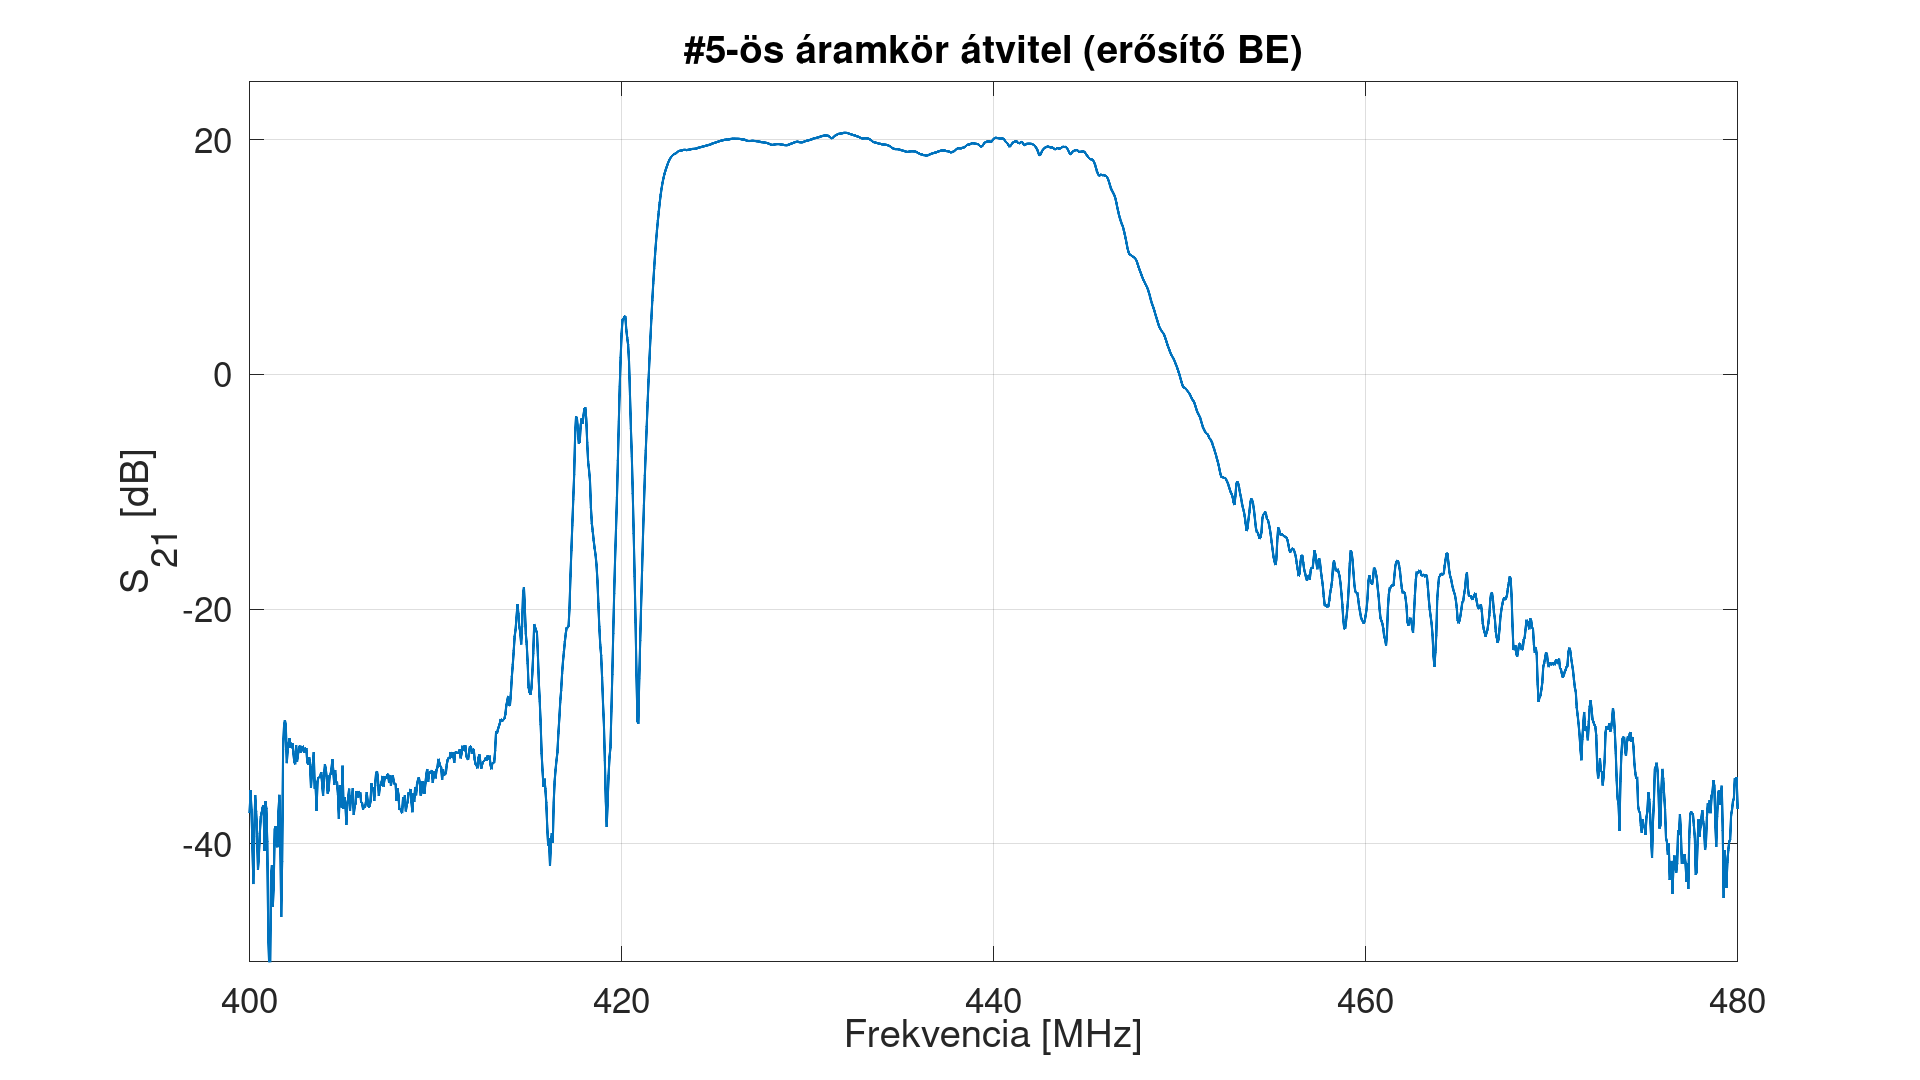
\includegraphics[keepaspectratio, width=\textwidth]{aramkor5_52.png}
	\caption{\#5-ös erősítő 400\,MHz - 480\,MHz, erősítő BE}
	\label{fig:meres52}
\end{figure}



\begin{figure}[!ht]
	\centering
	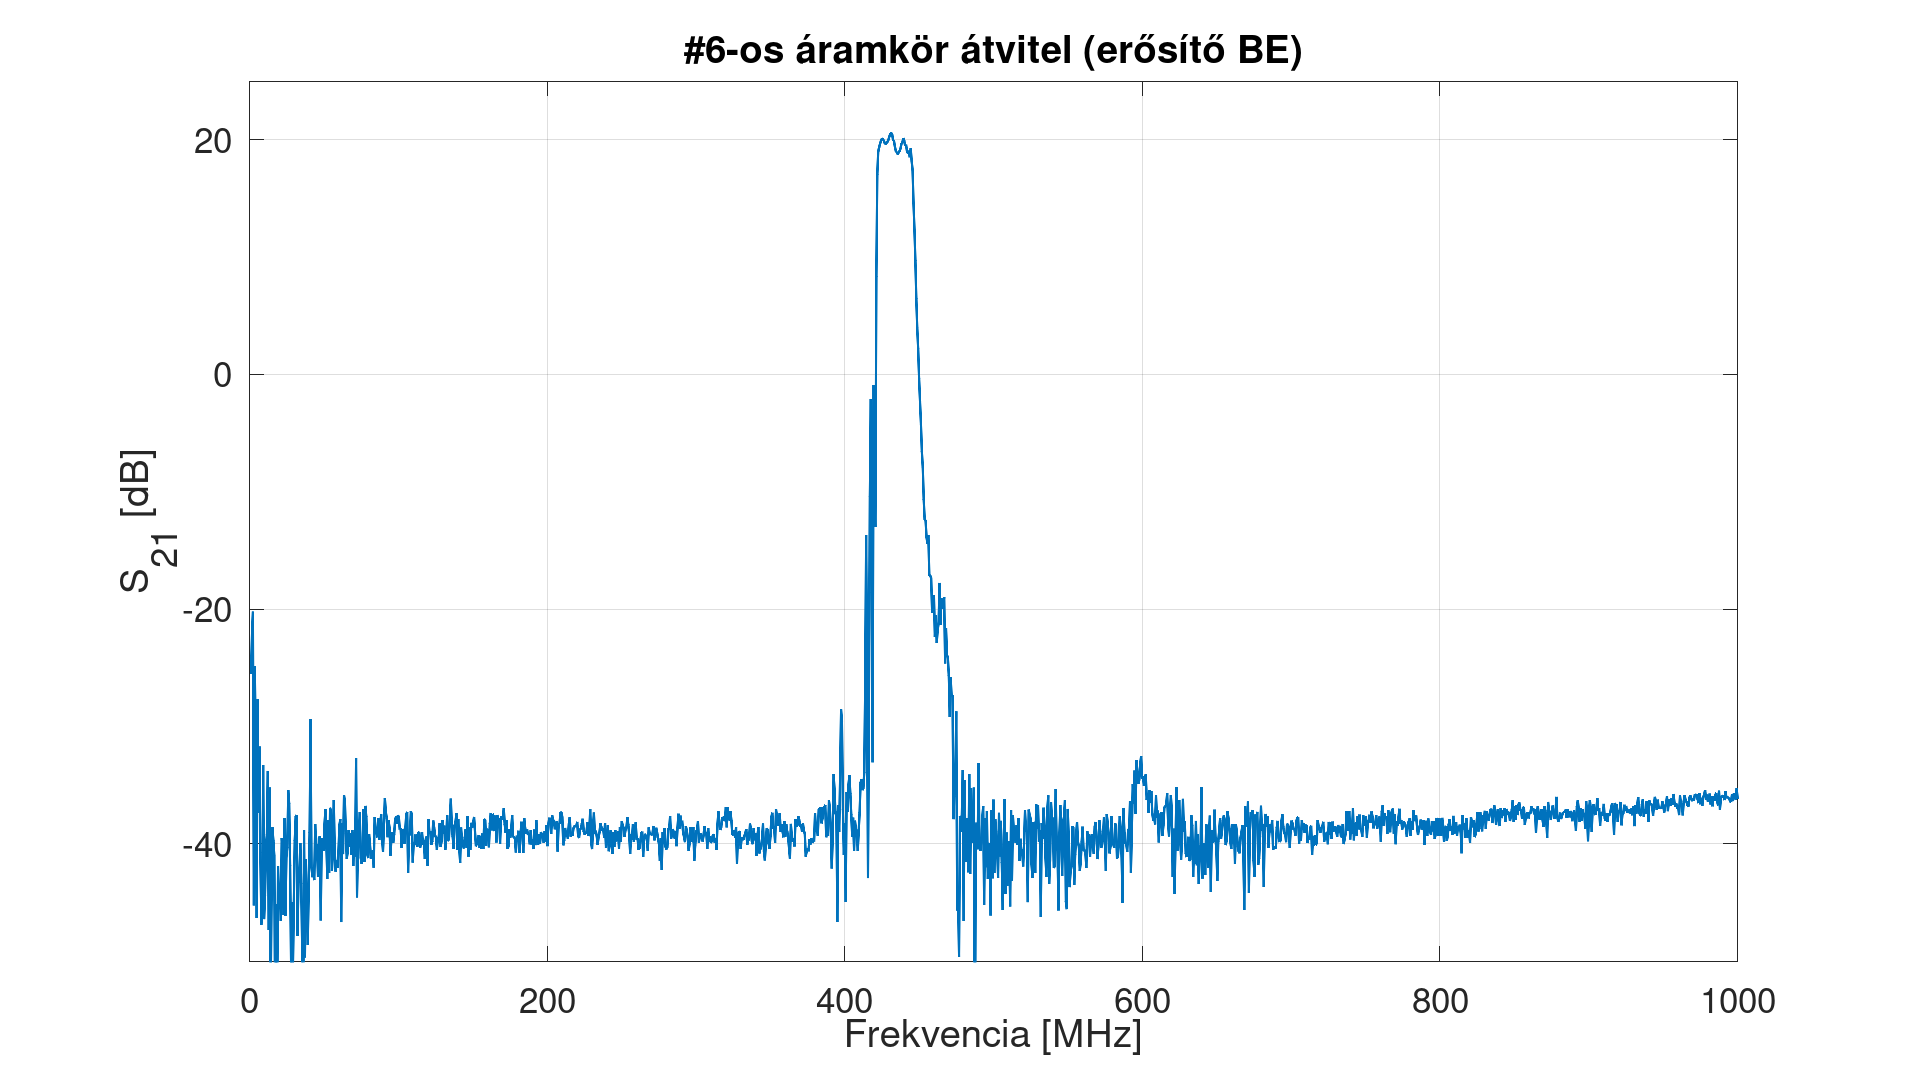
\includegraphics[keepaspectratio, width=\textwidth]{aramkor6_61.png}
	\caption{\#6-os erősítő 1\,MHz - 1\,GHz, erősítő BE}
	\label{fig:meres61}
\end{figure}

\begin{figure}[!ht]
	\centering
	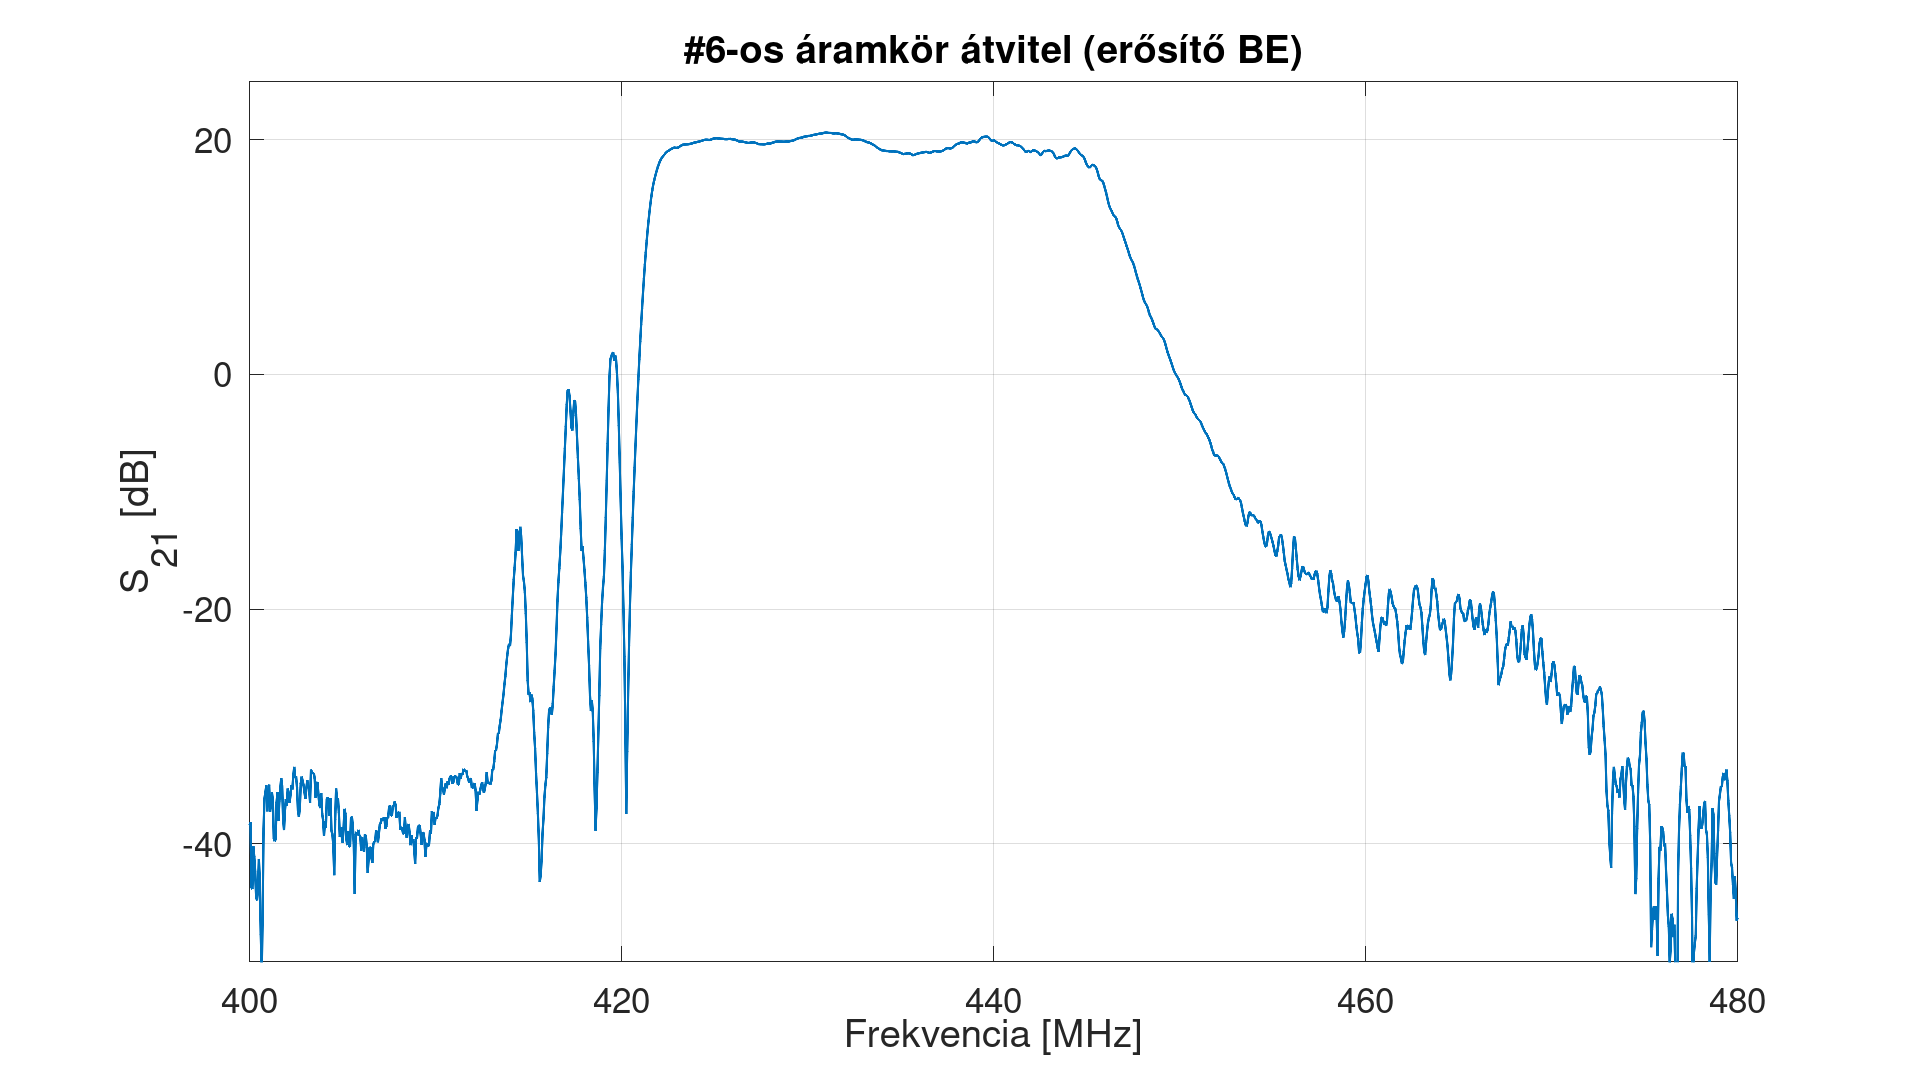
\includegraphics[keepaspectratio, width=\textwidth]{aramkor6_62.png}
	\caption{\#6-os erősítő 400\,MHz - 480\,MHz, erősítő BE}
	\label{fig:meres62}
\end{figure}



\begin{figure}[!ht]
	\centering
	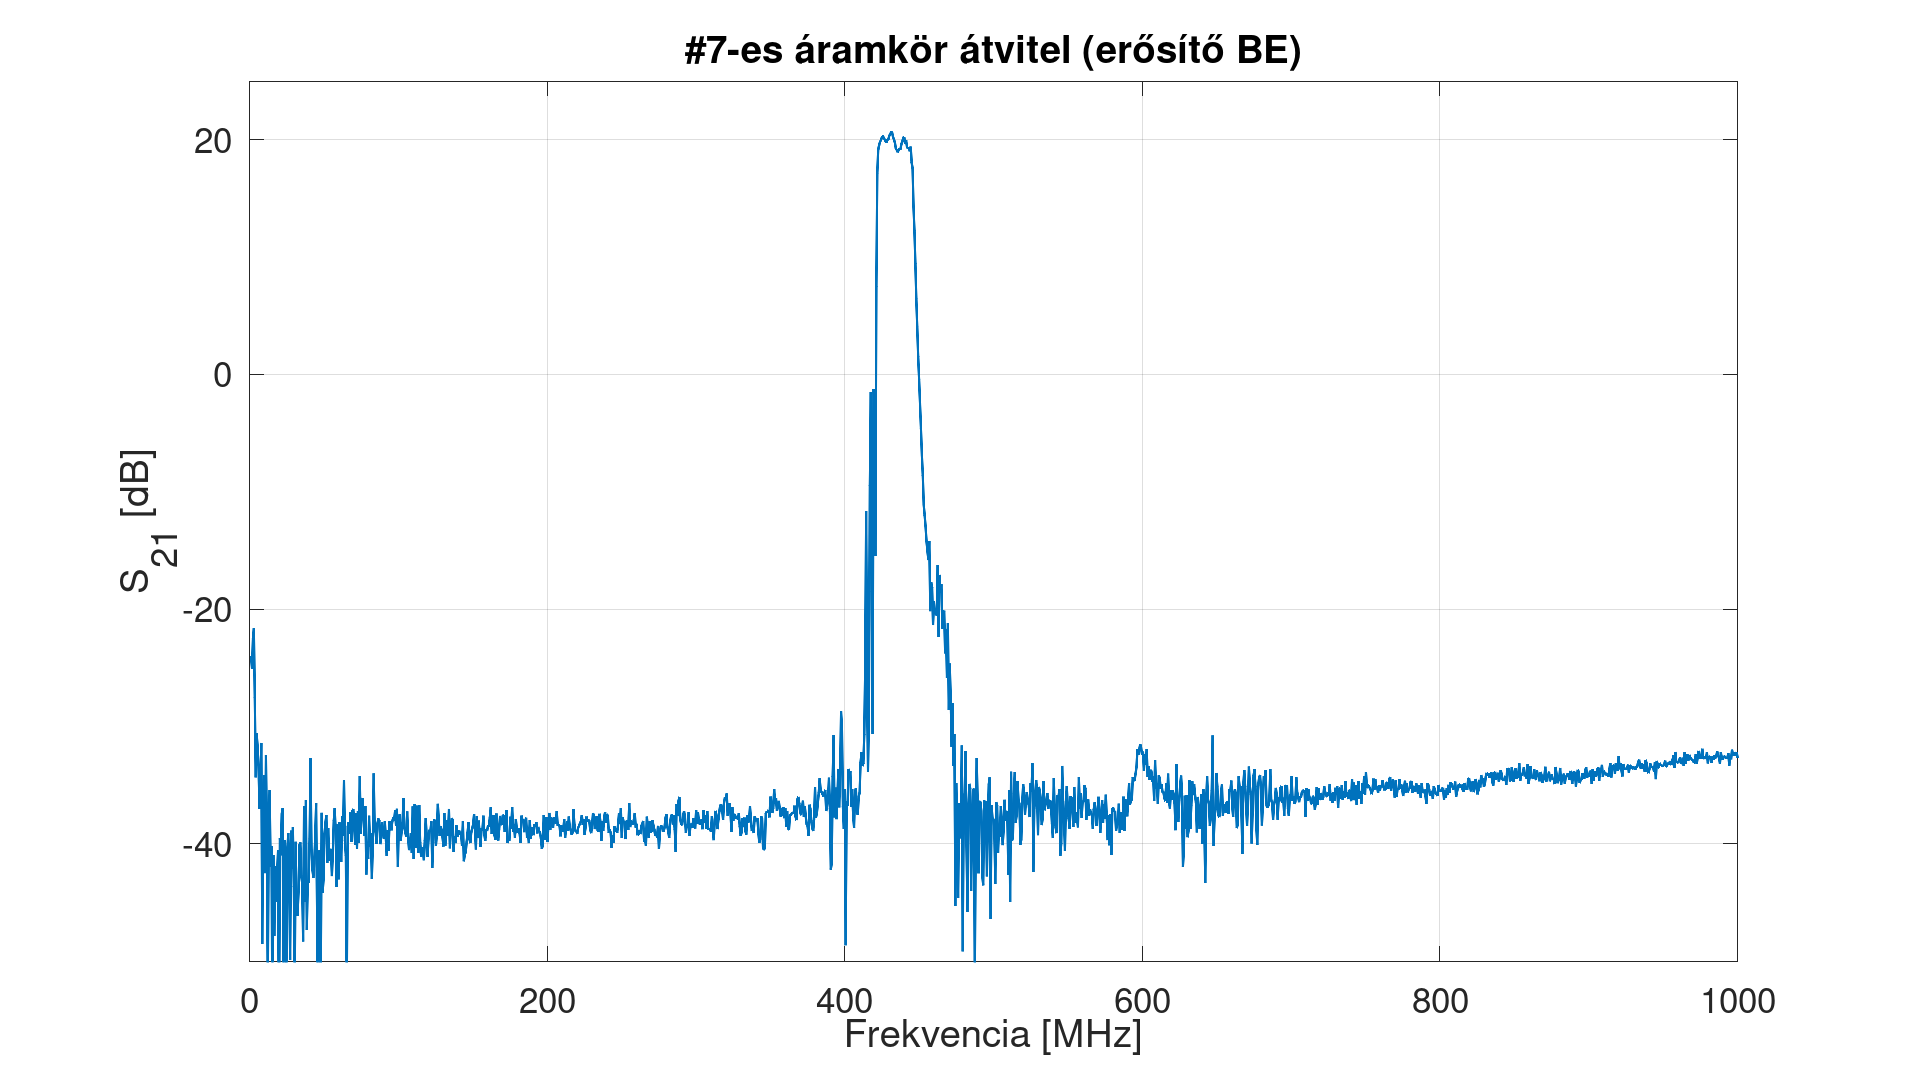
\includegraphics[keepaspectratio, width=\textwidth]{aramkor7_71.png}
	\caption{\#7-es erősítő 1\,MHz - 1\,GHz, erősítő BE}
	\label{fig:meres71}
\end{figure}

\begin{figure}[!ht]
	\centering
	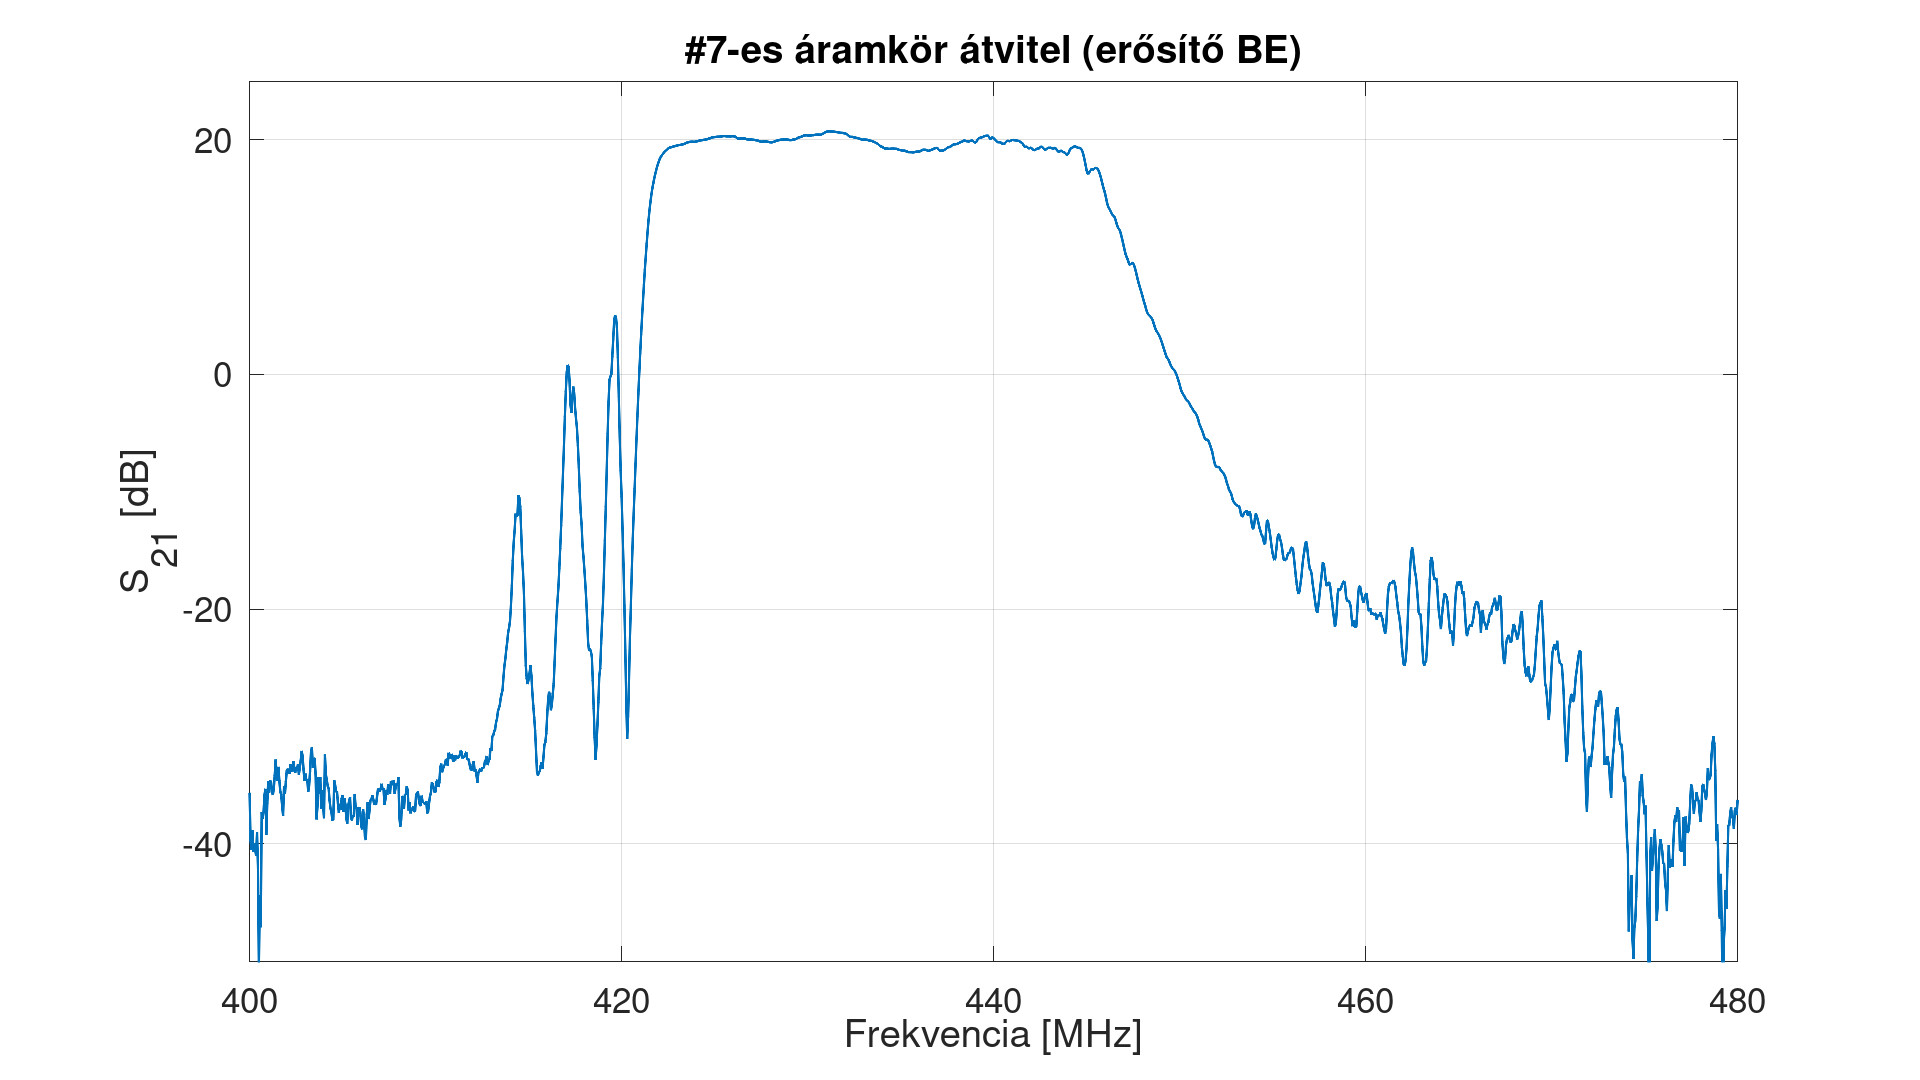
\includegraphics[keepaspectratio, width=\textwidth]{aramkor7_72.png}
	\caption{\#7-es erősítő 400\,MHz - 480\,MHz, erősítő BE}
	\label{fig:meres72}
\end{figure}



\begin{figure}[!ht]
	\centering
	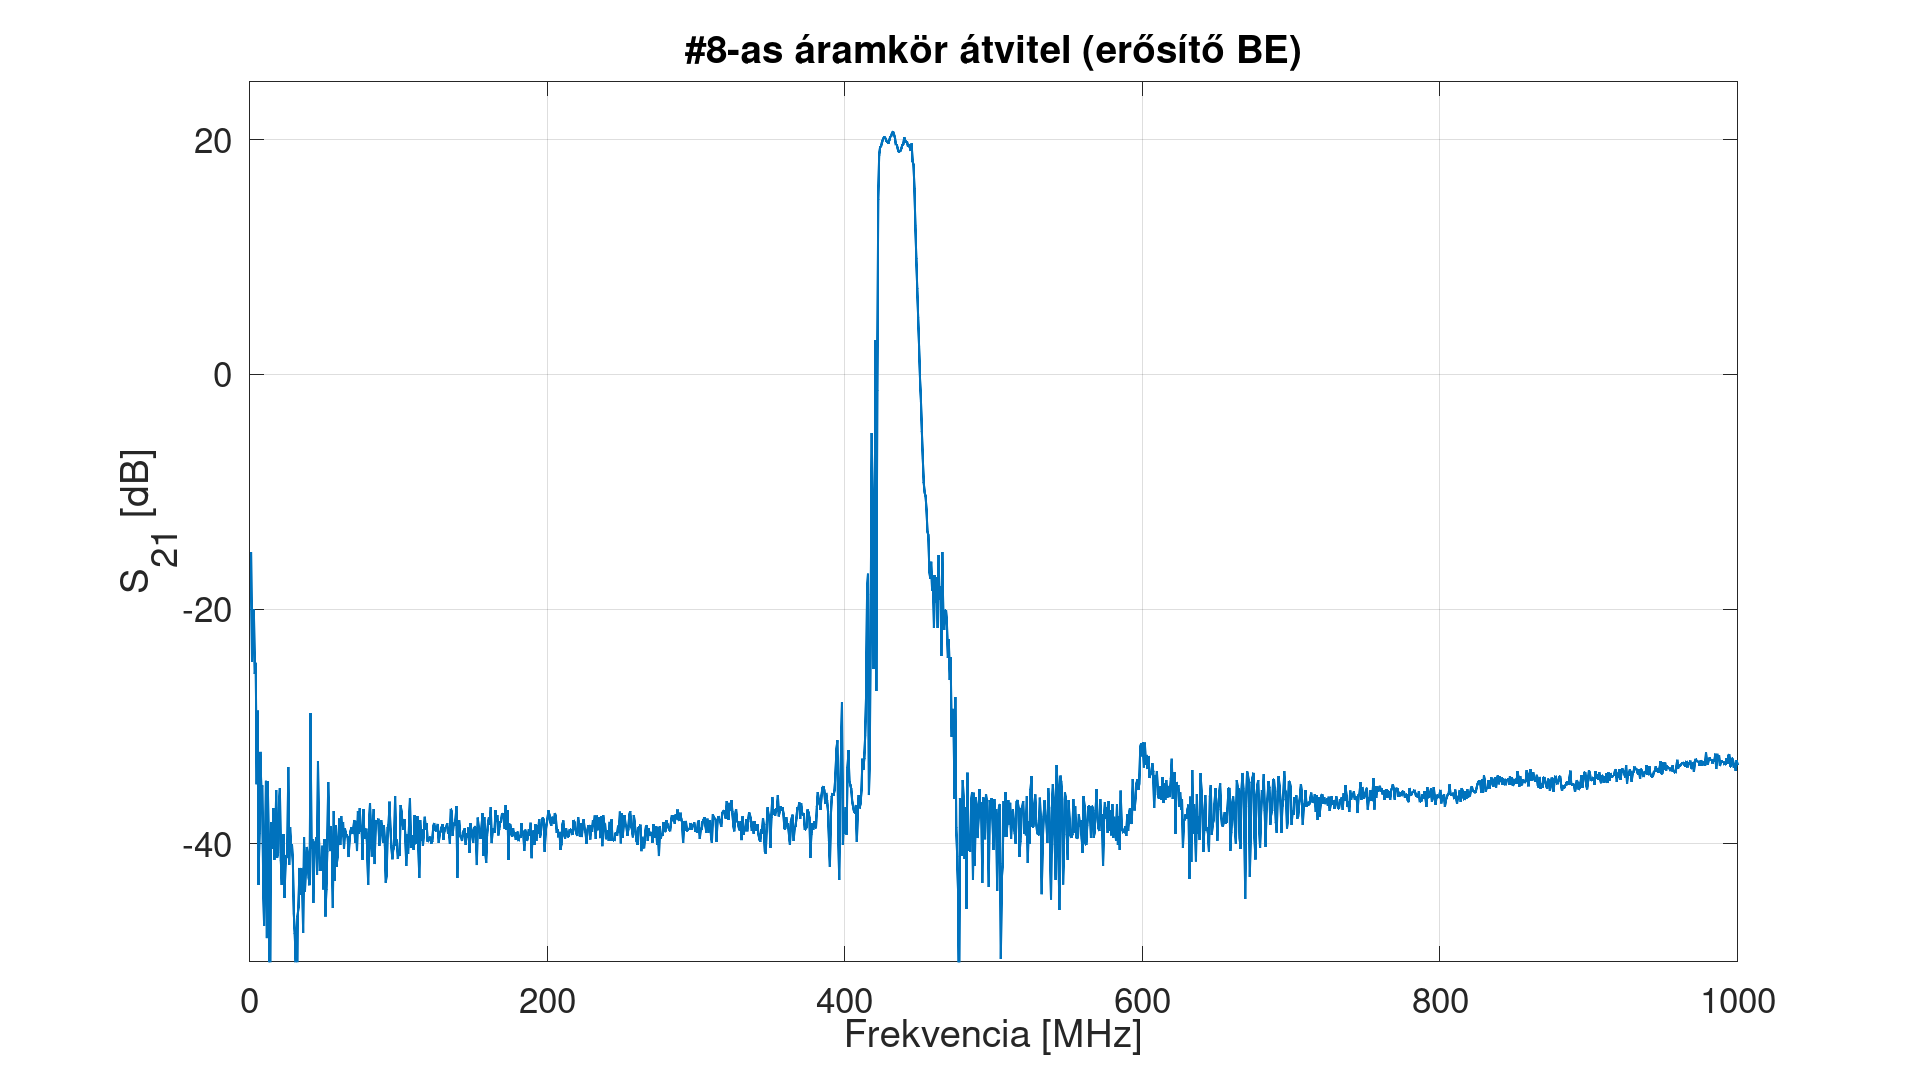
\includegraphics[keepaspectratio, width=\textwidth]{aramkor8_81.png}
	\caption{\#8-as erősítő 1\,MHz - 1\,GHz, erősítő BE}
	\label{fig:meres81}
\end{figure}

\begin{figure}[!ht]
	\centering
	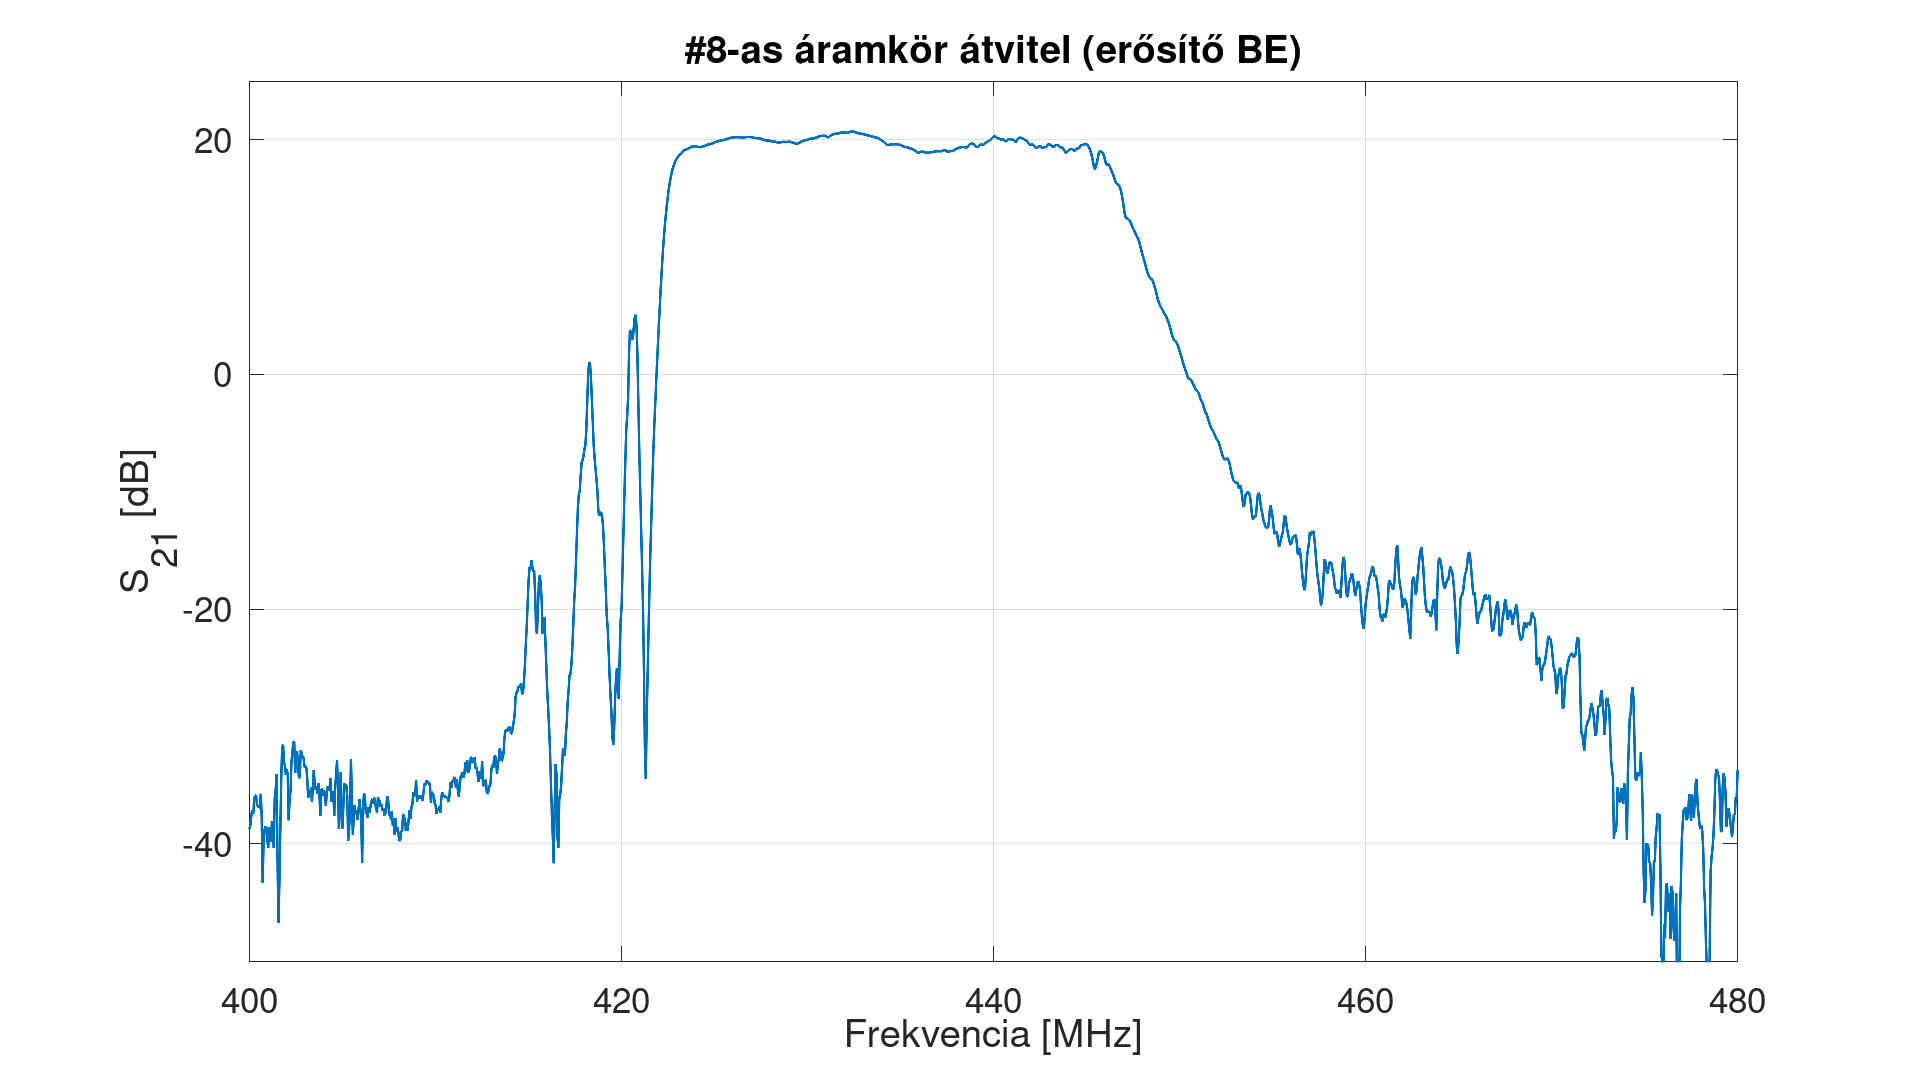
\includegraphics[keepaspectratio, width=\textwidth]{aramkor8_82.png}
	\caption{\#8-as erősítő 400\,MHz - 480\,MHz, erősítő BE}
	\label{fig:meres82}
\end{figure}
\newpage
